% !TeX program = pdflatex
% !TeX encoding = UTF-8
\documentclass[14pt,a4paper,oneside]{extreport}

% ================================================================
% Báo cáo học phần PROG2008 - Phát triển ứng dụng Web
% Compiler: pdfLaTeX, chạy ít nhất 2 lần để cập nhật mục lục.
% ================================================================


% Tự động tương thích cả pdfLaTeX và XeLaTeX / LuaLaTeX trên Overleaf
\usepackage{iftex}
\ifPDFTeX
  \usepackage[utf8]{vietnam}
  \usepackage{newtxtext,newtxmath}
\else
  \usepackage{fontspec}
  \defaultfontfeatures{Ligatures=TeX}
  \IfFontExistsTF{Times New Roman}{
    \setmainfont{Times New Roman}[
      BoldFont={Times New Roman Bold},
      ItalicFont={Times New Roman Italic},
      BoldItalicFont={Times New Roman Bold Italic}
    ]
  }{
    \IfFontExistsTF{DejaVu Serif}{
      \setmainfont{DejaVu Serif}
    }{
      \setmainfont{Latin Modern Roman}
    }
  }
\fi
\usepackage{geometry}
\geometry{a4paper,top=2.5cm,bottom=2.5cm,left=3cm,right=2cm,headsep=0.65cm,footskip=1cm}

\usepackage{setspace}
% Cỡ chữ 14 pt và giãn dòng 1.05 để cân bằng khả năng đọc với mục tiêu
% khoảng 35--40 trang; số trang còn phụ thuộc tỷ lệ ảnh thật được chèn.
\setstretch{1.05}
\setlength{\parindent}{1.27cm}
\setlength{\parskip}{0pt}
\setlength{\emergencystretch}{2em}
\usepackage{indentfirst}
\usepackage{microtype}

\usepackage{graphicx}
\usepackage{float}
\usepackage{pdflscape}
\usepackage{pdfpages}
\usepackage{longtable}
\usepackage{array}
\usepackage{tabularx}
\usepackage{ragged2e}
\usepackage{multirow}
\usepackage{enumitem}
\usepackage{titlesec}
\usepackage{fancyhdr}
\usepackage{caption}
\usepackage{xcolor}
\usepackage{tikz}
\usetikzlibrary{arrows.meta,calc,fit,positioning,shapes.geometric}
\usepackage{hyperref}
\usepackage{etoolbox}
\usepackage{xparse}
\usepackage{listings}

\definecolor{reportblue}{RGB}{0,102,204}
\definecolor{lightgray}{gray}{0.94}
\definecolor{midgray}{gray}{0.55}
\definecolor{darkgray}{gray}{0.20}

% Bảng theo mẫu báo cáo cũ: đường viền kín, nét đều, khoảng đệm thoáng.
\setlength{\arrayrulewidth}{0.6pt}
\setlength{\tabcolsep}{5pt}
\renewcommand{\arraystretch}{1.25}

\hypersetup{
  unicode=true,
  colorlinks=false,
  hidelinks,
  pdfborder={0 0 0},
  pdfauthor={Nhóm sinh viên học phần PROG2008},
  pdftitle={Báo cáo bài tập lớn học phần Phát triển ứng dụng Web}
}
\urlstyle{same}
\PassOptionsToPackage{hyphens}{url}
\makeatletter
\g@addto@macro\UrlBreaks{%
  \do\/\do\-\do\_\do\:\do\.\do\=\do\?\do\&\do\%\do\#\do\+\do\@%
}
\makeatother

% ================================================================
% Định dạng tiêu đề, mục lục và caption
% ================================================================
\renewcommand{\chaptername}{CHƯƠNG}
\titleformat{\chapter}[block]
  {\centering\bfseries\fontsize{18pt}{22pt}\selectfont}
  {\chaptername~\thechapter.}
  {0.7em}
  {\MakeUppercase}
\titlespacing*{\chapter}{0pt}{20pt}{15pt}

\titleformat{\section}
  {\bfseries\fontsize{16pt}{19pt}\selectfont}
  {\thesection.}{0.7em}{}
\titleformat{\subsection}
  {\bfseries\fontsize{14pt}{17pt}\selectfont}
  {\thesubsection.}{0.7em}{}
\titleformat{\subsubsection}
  {\bfseries\itshape\fontsize{14pt}{17pt}\selectfont}
  {\thesubsubsection.}{0.7em}{}

\titlespacing*{\section}{0pt}{1.0em}{0.5em}
\titlespacing*{\subsection}{0pt}{0.8em}{0.4em}
\titlespacing*{\subsubsection}{0pt}{0.7em}{0.3em}

\renewcommand{\contentsname}{MỤC LỤC}
\renewcommand{\listtablename}{DANH MỤC BẢNG}
\renewcommand{\listfigurename}{DANH MỤC HÌNH}
\renewcommand{\tablename}{Bảng}
\renewcommand{\figurename}{Hình}
\renewcommand{\bibname}{TÀI LIỆU THAM KHẢO}
\setcounter{tocdepth}{3}
\setcounter{secnumdepth}{3}

\captionsetup{font=normalsize,labelfont=bf,justification=centering}
\captionsetup[table]{position=top,skip=6pt}
\captionsetup[figure]{position=bottom,skip=6pt}

\setlist[itemize]{leftmargin=1.1cm,label=--,itemsep=0.2em,topsep=0.3em}
\setlist[enumerate]{leftmargin=1.1cm,itemsep=0.2em,topsep=0.3em}

\lstdefinestyle{reportcode}{
  basicstyle=\ttfamily\small,
  numbers=left,
  numberstyle=\scriptsize,
  frame=single,
  backgroundcolor=\color{lightgray},
  breaklines=true,
  showstringspaces=false,
  tabsize=2,
  columns=fullflexible
}

% ================================================================
% Header, footer và đánh số trang theo mẫu báo cáo cũ
% ================================================================
\pagestyle{fancy}
\fancyhf{}
\fancyhead[L]{\small Trường Đại học CMC}
\fancyhead[R]{\small Học phần: PROG2008}
\fancyfoot[C]{\thepage}
\renewcommand{\headrulewidth}{0.4pt}
\setlength{\headheight}{17pt}
\fancypagestyle{plain}{
  \fancyhf{}
  \fancyhead[L]{\small Trường Đại học CMC}
  \fancyhead[R]{\small Học phần: PROG2008}
  \fancyfoot[C]{\thepage}
  \renewcommand{\headrulewidth}{0.4pt}
}

% ================================================================
% Lệnh chèn ảnh trung thực: nếu chưa có file thì hiện khung giữ chỗ.
% Khi đã chụp ảnh, chỉ cần lưu đúng đường dẫn; không sửa nội dung báo cáo.
% ================================================================
\NewDocumentCommand{\ReportImage}{O{0.28\textheight} m m m m}{%
  \begin{figure}[H]
    \centering
    \IfFileExists{#2}{%
      \includegraphics[width=0.96\linewidth,height=#1,keepaspectratio]{#2}%
    }{%
      \fbox{%
        \begin{minipage}[c][#1][c]{0.91\linewidth}
          \centering
          \textbf{VỊ TRÍ CHÈN ẢNH MINH CHỨNG}\\[0.5em]
          \texttt{\detokenize{#2}}\\[0.5em]
          \small #5\\[0.5em]
          \textit{Không sử dụng ảnh minh họa giả.}
        \end{minipage}%
      }%
    }
    \caption{#3\label{#4}}
  \end{figure}
}

\newcommand{\BlankField}[1]{\textit{[#1]}}
% nolinkurl giữ kiểu monospace nhưng cho phép ngắt dòng tại dấu /, . và -.
\newcommand{\CodePath}[1]{\nolinkurl{#1}}
% Đối số 1 là một lệnh URL trong metadata.tex, ví dụ \WebsiteURL.
\newcommand{\OptionalURL}[2]{%
  \ifdefempty{#1}{\BlankField{#2}}{\expandafter\url\expandafter{#1}}%
}

% ================================================================
% THÔNG TIN CẦN XÁC NHẬN TRƯỚC KHI NỘP
% Chỉ sửa các lệnh trong file này; không cần tìm trong toàn bộ báo cáo.
% ================================================================

\newcommand{\UniversityName}{TRƯỜNG ĐẠI HỌC CMC}
\newcommand{\FacultyName}{KHOA CÔNG NGHỆ THÔNG TIN VÀ TRUYỀN THÔNG}
\newcommand{\CourseName}{CÔNG NGHỆ PHẦN MỀM}
\newcommand{\CourseCode}{INFO2011}
\newcommand{\InstructorName}{Phạm Tuấn Anh}
\newcommand{\ClassCode}{N02}
\newcommand{\ProjectTitle}{WEB ĐỌC TRUYỆN CHỮ ONLINE-CMC TRUYỆN}
\newcommand{\AcademicYear}{2025--2026}
\newcommand{\SubmissionPlace}{Hà Nội}
\newcommand{\SubmissionYear}{2026}

% Các URL minh chứng dự án
\newcommand{\WebsiteURL}{https://cmc-truyen.vercel.app}
\newcommand{\SourceCodeURL}{https://github.com/suzynotsusie/cmc-truyen-temp}
\newcommand{\DemoVideoURL}{https://youtu.be/demo-cmc-truyen}

% Danh sách chính thức của nhóm gồm 4 thành viên (Trần Thị Kim Uyên - Nhóm trưởng).

\newcommand{\StudentOneName}{Nguyễn Thị Thùy}
\newcommand{\StudentOneId}{BAI252513}
\newcommand{\StudentTwoName}{Trần Thị Kim Uyên}
\newcommand{\StudentTwoId}{BAI250072}
\newcommand{\StudentThreeName}{Nguyễn Hải Dương}
\newcommand{\StudentThreeId}{BAI250020}
\newcommand{\StudentFourName}{Nguyễn Tuấn Thành}
\newcommand{\StudentFourId}{BAI252417}
\newcommand{\StudentFiveName}{Vũ Viết Trí}
\newcommand{\StudentFiveId}{BAI250063}
% Phân công công việc chi tiết của từng thành viên
\newcommand{\TaskOne}{{Điều phối hoạt động nhóm, quản lý backlog, phân chia nhiệm vụ, tổng hợp yêu cầu và review báo cáo; phụ trách thiết kế UI/UX phía người dùng, xây dựng trang
chủ, trang chi tiết truyện, luồng đọc truyện và lịch sử đọc; phát triển chức năng phân trang và sắp xếp dữ liệu phía Backend; xây dựng kịch bản kiểm thử người dùng, thực hiện kiểm thử tích hợp và nghiệm thu tính năng.}}
\newcommand{\TaskTwo}{{Thiết kế PostgreSQL schema và migration; xây dựng các chức năng CRUD cho dữ liệu người dùng, truyện, chương, bình luận và các thực thể liên quan; thực hiện kiểm tra quyền truy cập, quyền sở hữu và tính hợp lệ của dữ liệu; phát triển Google OAuth/OTP, AI service, API upload Supabase và tính năng collaborator; tối ưu truy vấn, bảo đảm tính toàn vẹn dữ liệu, kiểm thử tầng database và soạn thảo tài liệu ERD.}}
\newcommand{\TaskThree}{{Phát triển các chức năng Frontend cho bình luận, theo dõi, đánh giá và thông báo; xử lý giao diện responsive trên nhiều kích thước màn hình; xây dựng chức năng Backend phục vụ hiển thị chi tiết truyện, chương, bình luận, đánh giá và lịch sử đọc; thực hiện validation dữ liệu, tích hợp API và đồng bộ dữ liệu giữa Frontend--Backend.}}
\newcommand{\TaskFour}{{ Phụ trách thiết kế kiến trúc và phát triển hệ thống Backend, bao gồm authentication, JWT, RBAC, moderation, notification, audit log và Redis/BullMQ worker; xây dựng chức năng tìm kiếm và lọc dữ liệu truyện; phát triển logic cá nhân hóa và quản lý lịch sử đọc; tối ưu hiệu năng và tốc độ phản hồi API; cấu hình server, thiết lập CI/CD, logging, kiểm thử Backend và viết tài liệu kỹ thuật.}}
\newcommand{\TaskFive}{{Phụ trách thiết kế và phát triển giao diện dành cho Admin và Moderator, bao gồm dashboard, quản lý người dùng, truyện, báo cáo, bình luận, hồ sơ và audit log; xây dựng loading state, error state và route guard; thực hiện kiểm thử component, kiểm thử giao diện và kiểm thử phân quyền trên các màn hình quản trị.}}

\begin{document}

% Trang 1: bìa; trang 2: phân công công việc.
\pagenumbering{gobble}
\pagestyle{empty}
% !TeX encoding = UTF-8
% Trang bìa chuyển từ main.tex trong mau.zip, dùng thông tin của báo cáo hiện tại.
\begin{titlepage}
  \thispagestyle{empty}

  \begin{tikzpicture}[remember picture,overlay]
    \draw[line width=3pt,color=reportblue!80]
      ([xshift=1.2cm,yshift=-1.2cm]current page.north west)
      rectangle
      ([xshift=-1.2cm,yshift=1.2cm]current page.south east);
    \draw[line width=1pt,color=reportblue!40]
      ([xshift=1.45cm,yshift=-1.45cm]current page.north west)
      rectangle
      ([xshift=-1.45cm,yshift=1.45cm]current page.south east);
  \end{tikzpicture}

  \centering
  \textbf{\large BỘ GIÁO DỤC VÀ ĐÀO TẠO}\\[4pt]
  \textbf{\large \UniversityName}

  \vspace{0.5cm}
  \IfFileExists{images/cmc_logo.png}
    {
\includegraphics[width=8cm]{images/cmc_logo.png}}
    {\fbox{\parbox[c][2.8cm][c]{8cm}{%
      \centering Đặt file \texttt{cmc\_logo.png} trong thư mục \texttt{images}}}}

  \vspace{1cm}
  \textbf{\LARGE BÁO CÁO BÀI TẬP LỚN}\\[12pt]
  \textbf{\large HỌC PHẦN: \CourseName\ (\CourseCode)}

  \vspace{1.5cm}
  \textbf{\Large Tên đề tài:}\\[8pt]
  \textbf{\LARGE \ProjectTitle}

  \vspace{1.5cm}
  \begin{flushleft}
    \hspace{3.5cm}\textbf{Giảng viên:} \InstructorName\\[4pt]
    \hspace{3.5cm}\textbf{Mã lớp học phần:} \ClassCode\\[8pt]
    \hspace{3.5cm}\textbf{Nhóm sinh viên:}
  \end{flushleft}

  \begin{center}
    \begin{tabular}{cll}
      1. & \StudentOneName  & \StudentOneId\\[4pt]
      2. & \StudentTwoName  & \StudentTwoId\\[4pt]
      3. & \StudentThreeName &\StudentThreeId\\[4pt]
      4. & \StudentFourName & \StudentFourId\\[4pt]
      5. & \StudentFiveName & \StudentFiveId\\
    \end{tabular}
  \end{center}

  \vfill
  \textbf{\large \SubmissionPlace, tháng 7 -- \SubmissionYear}
\end{titlepage}

\clearpage
\thispagestyle{empty}
\begin{center}
  {\bfseries\fontsize{18pt}{22pt}\selectfont PHÂN CÔNG CÔNG VIỆC}
\end{center}

\vspace{0.7cm}
\noindent
\begin{longtable}{|>{\centering\arraybackslash}p{1.0cm}|
                  >{\RaggedRight\arraybackslash}p{3.4cm}|
                  >{\centering\arraybackslash}p{2.6cm}|
                  >{\RaggedRight\arraybackslash}p{7.0cm}|}
\hline
\textbf{STT} & \textbf{Họ và tên} & \textbf{Mã sinh viên} & \textbf{Nội dung phụ trách} \\
\hline
1 & \StudentOneName & \StudentOneId & \TaskOne \\
\hline
2 & \StudentTwoName & \StudentTwoId & \TaskTwo \\
\hline
3 & \StudentThreeName & \StudentThreeId & \TaskThree \\
\hline
4 & \StudentFourName & \StudentFourId & \TaskFour \\
\hline
5 & \StudentFiveName & \StudentFiveId & \TaskFive \\
\hline
\end{longtable}






% Phần đầu dùng số La Mã; danh mục bảng đặt trên danh mục hình.
\clearpage
\pagenumbering{roman}
\setcounter{page}{1}
\pagestyle{fancy}
\tableofcontents
\clearpage
\phantomsection
\addcontentsline{toc}{chapter}{\listtablename}
\listoftables
\clearpage
\phantomsection
\addcontentsline{toc}{chapter}{\listfigurename}
\listoffigures
\clearpage
\chapter*{DANH MỤC TỪ VIẾT TẮT}
\addcontentsline{toc}{chapter}{Danh mục từ viết tắt}

\begin{longtable}{|>{\bfseries}p{0.20\textwidth}|p{0.70\textwidth}|}
\hline
AI & Artificial Intelligence -- Trí tuệ nhân tạo \\
\hline
API & Application Programming Interface -- Giao diện lập trình ứng dụng \\
\hline
CSDL & Cơ sở dữ liệu \\
\hline
CSS & Cascading Style Sheets \\
\hline
DOM & Document Object Model \\
\hline
FE & Frontend -- Phần giao diện phía người dùng \\
\hline
BE & Backend -- Phần xử lý phía máy chủ \\
\hline
HTML & HyperText Markup Language \\
\hline
HTTP & HyperText Transfer Protocol \\
\hline
JWT & JSON Web Token \\
\hline
RBAC & Role-Based Access Control -- Kiểm soát truy cập theo vai trò \\
\hline
REST & Representational State Transfer \\
\hline
SPA & Single-Page Application -- Ứng dụng web một trang \\
\hline
SQL & Structured Query Language \\
\hline
UI/UX & User Interface/User Experience -- Giao diện/Trải nghiệm người dùng \\
\hline
URL & Uniform Resource Locator \\
\hline
\end{longtable}


% Nội dung chính dùng số Ả Rập, bắt đầu từ Chương 1.
\clearpage
\pagenumbering{arabic}
\setcounter{page}{1}

\chapter{GIỚI THIỆU BÀI TOÁN}
\label{chap:introduction}

\section{Bối cảnh và động cơ thực hiện}

Nhu cầu đọc truyện trực tuyến ngày càng gắn với khả năng tìm kiếm nhanh, tiếp tục đúng vị trí đã đọc và sử dụng ổn định trên nhiều thiết bị. Khi số lượng truyện, chương, bình luận và báo cáo tăng, cách quản lý thủ công dễ phát sinh chậm trễ, sai sót và khó truy vết.

Từ thực tế đó, nhóm xây dựng ứng dụng web \textbf{CMC Truyện}. Hệ thống hướng đến hai mục tiêu chính: tạo trải nghiệm đọc thuận tiện cho người dùng và cung cấp quy trình đăng tải, kiểm duyệt, quản trị nội dung rõ ràng cho đội ngũ vận hành.

\section{Phát biểu bài toán}

\subsection{Vấn đề của người đọc}
Các vấn đề chính của người đọc gồm:
\begin{itemize}[leftmargin=4.5em, label=--, labelsep=0.6em]

  \item Khó tìm kiếm và chọn truyện khi dữ liệu tăng;
  \item Không đồng bộ lịch sử, vị trí đọc và truyện đang theo dõi;
  \item Thiếu tùy chỉnh hiển thị và thông báo chương mới;
  \item Bình luận rác hoặc nội dung vi phạm làm giảm chất lượng cộng đồng.
\end{itemize}


\subsection{Vấn đề của người đăng nội dung và đội ngũ vận hành}

Người đăng nội dung cần quản lý truyện, chương và theo dõi trạng thái kiểm duyệt. Người kiểm duyệt cần xử lý hàng chờ, báo cáo vi phạm và phản hồi cho người đăng. Quản trị viên cần quản lý tài khoản, vai trò, nội dung và nhật ký thao tác. Vì vậy, hệ thống không chỉ thực hiện các chức năng thêm, sửa, xóa mà còn phải bảo đảm xác thực, phân quyền, quy trình trạng thái và khả năng truy vết.
\clearpage
\section{Mục tiêu của hệ thống}

\begin{table}[htbp]
\centering
\caption{Mục tiêu của hệ thống}
\label{tab:system-objectives}
\begin{tabularx}{\textwidth}{|>{\centering\arraybackslash}p{1.2cm}|>{\RaggedRight\arraybackslash}p{5.2cm}|X|}
\hline
\textbf{Mã} & \textbf{Mục tiêu} & \textbf{Kết quả mong đợi} \\
\hline
M1 & Cung cấp trải nghiệm khám phá và đọc truyện thuận tiện & Có trang tìm kiếm, chi tiết truyện, đọc chương, bảng xếp hạng và URL định danh theo slug. \\
\hline
M2 & Cá nhân hóa trải nghiệm người dùng & Có lịch sử đọc, chương đã đọc, theo dõi truyện, thông báo và tùy chọn đọc. \\
\hline
M3 & Bảo đảm quy trình xuất bản có kiểm duyệt & Truyện mới của Uploader ở trạng thái chờ; Moderator/Admin có thể duyệt, yêu cầu sửa hoặc từ chối. \\
\hline
M4 & Bảo vệ thao tác theo đúng thẩm quyền & JWT xác thực phiên; middleware RBAC bảo vệ route; frontend có route guard tương ứng. \\
\hline
M5 & Hỗ trợ quản trị và truy vết & Có quản lý người dùng, truyện, báo cáo, từ khóa nhạy cảm và audit log. \\
\hline
M6 & Có khả năng kiểm chứng chất lượng kỹ thuật & Có kiểm thử backend, frontend và quy trình build production; kết quả thực chạy được trình bày ở Chương~\ref{chap:implementation}. \\
\hline
\end{tabularx}
\end{table}

Báo cáo mô tả hệ thống tại thời điểm hoàn thiện sản phẩm. Kết quả được ghi nhận dựa trên mã nguồn, kiểm thử, bản build và minh chứng vận hành tương ứng.

\clearpage
\section{Đối tượng sử dụng và bên liên quan}

\begin{figure}[H]
\centering
\begin{tikzpicture}[
  actor/.style={
    draw,
    rounded corners,
    minimum width=2.45cm,
    minimum height=0.85cm,
    align=center,
    font=\small
  },
  system/.style={
    draw,
    double,
    very thick,
    minimum width=5.2cm,
    minimum height=3.4cm,
    align=center
  },
  arrow/.style={-{Latex[length=2.4mm]},thick}
]
\node[system] (sys) {
  \textbf{CMC Truyện}\\[0.4em]
  Khám phá và đọc\\
  Cá nhân hóa\\
  Đăng nội dung\\
  Kiểm duyệt và quản trị
};
\node[actor,left=1.8cm of sys,yshift=1.7cm] (guest) {Guest};
\node[actor,left=1.8cm of sys] (user) {User};
\node[actor,left=1.8cm of sys,yshift=-1.7cm] (uploader) {Uploader};
\node[actor,right=1.8cm of sys,yshift=1.15cm] (moderator) {Moderator};
\node[actor,right=1.8cm of sys,yshift=-1.15cm] (admin) {Admin};
\draw[arrow] (guest) -- (sys);
\draw[arrow] (user) -- (sys);
\draw[arrow] (uploader) -- (sys);
\draw[arrow] (moderator) -- (sys);
\draw[arrow] (admin) -- (sys);
\end{tikzpicture}
\caption{Sơ đồ ngữ cảnh và các tác nhân chính}
\label{fig:system-context}
\end{figure}

Hình~\ref{fig:system-context} khái quát năm nhóm tác nhân tương tác với hệ thống. Trong đó, Guest là người chưa đăng nhập, không phải một vai trò được lưu trong bảng \CodePath{users}.

\begin{table}[H]
\centering
\caption{Đối tượng sử dụng và nhu cầu chính}
\label{tab:stakeholders}
\small
\renewcommand{\arraystretch}{1.08}
\begin{tabularx}{\textwidth}{|>{\bfseries\RaggedRight\arraybackslash}p{2.7cm}|X|X|}
\hline
\textbf{Đối tượng} & \textbf{Nhu cầu} & \textbf{Giá trị hệ thống cung cấp} \\
\hline
Guest & Khám phá nội dung trước khi đăng ký & Xem trang chủ, tìm kiếm, bảng xếp hạng, thông tin truyện và nội dung công khai. \\
\hline
User & Đọc lâu dài và tương tác & Lưu lịch sử, theo dõi, đánh giá, bình luận, nhận thông báo và tùy chỉnh trải nghiệm đọc. \\
\hline
Uploader & Đưa nội dung lên hệ thống & Tạo và chỉnh sửa truyện, nhập nội dung, quản lý chương và cộng tác viên theo quy trình duyệt. \\
\hline
Moderator & Duy trì chất lượng nội dung & Duyệt truyện chờ và xử lý báo cáo, bình luận hoặc hồ sơ theo phạm vi được giao. \\
\hline
Admin & Quản trị toàn hệ thống & Quản lý người dùng, vai trò, truyện, báo cáo, từ khóa, nhật ký và số liệu tổng quan. \\
\hline
Nhóm phát triển & Bảo trì và mở rộng sản phẩm & Duy trì kiến trúc, API, cơ sở dữ liệu, kiểm thử, tài liệu và cấu hình triển khai. \\
\hline
\end{tabularx}
\end{table}
\clearpage
\section{Phạm vi chức năng}

\subsection{Chức năng trong phạm vi}

Phạm vi chức năng được xác định từ yêu cầu dự án, route frontend và router backend \cite{requirements}, gồm:

\begin{itemize}[leftmargin=4.5em, label=--, labelsep=0.6em]
  \item Xác thực và tài khoản: Đăng ký, đăng nhập, đăng xuất, Google OAuth, quên/đặt lại mật khẩu bằng OTP và cập nhật hồ sơ;
  \item Khám phá truyện: Danh sách, tìm kiếm, lọc theo tag hoặc danh mục, bảng xếp hạng và trang chi tiết;
  \item Trải nghiệm đọc: Đọc chương theo URL thân thiện, lưu lịch sử, lưu chương đã đọc và tùy chọn hiển thị;
  \item Mở khóa chương trả phí: Hiển thị số dư Tinh thạch, kiểm tra quyền đọc, mở khóa chương bằng số dư nội bộ và lưu lịch sử giao dịch;
  \item Tương tác: Theo dõi, đánh giá sao, bình luận, trả lời, bình chọn và báo cáo vi phạm;
  \item Đăng nội dung: Tạo truyện, import tệp văn bản/EPUB, quản lý chương, tag và cộng tác viên;
  \item Kiểm duyệt: Hàng chờ truyện, yêu cầu sửa, từ chối/duyệt, xử lý bình luận, hồ sơ và báo cáo;
  \item Quản trị: Quản lý user, role, trạng thái tài khoản, truyện, từ khóa, báo cáo và audit log;
  \item Tính năng hỗ trợ: Tóm tắt chương và gợi ý truyện bằng AI, notification, worker và hàng đợi tác vụ nền.
\end{itemize}


\subsection{Ngoài phạm vi hoặc chưa đủ minh chứng}

Các nội dung ngoài phạm vi hoặc chưa đủ bằng chứng gồm:

\begin{itemize}[leftmargin=4.5em, label=--, labelsep=0.6em]
  \item Thanh toán, gói thuê bao, quảng cáo, bản quyền nội dung và chia sẻ doanh thu;
  \item Nạp Tinh thạch hoặc thanh toán qua cổng thanh toán thật; hệ thống hiện chỉ cấp số dư demo và ghi nhận giao dịch mở khóa nội bộ.
  \item Ứng dụng di động native hoặc chế độ đọc ngoại tuyến;
  \item Kiểm thử tải, kiểm thử xâm nhập và chỉ số SLA trên môi trường production;
  \item Khả năng chịu lỗi của Redis/worker và tính đúng đắn của hàng đợi khi hệ thống khởi động lại;
  \item Liên kết website production, video demo và dashboard giám sát thực tế;
  \item Số liệu người dùng thật, dữ liệu vận hành thật hoặc kết quả kinh doanh.
\end{itemize}



\section{Yêu cầu phi chức năng}

\begin{table}[H]
\centering
\caption{Yêu cầu phi chức năng và giải pháp đáp ứng}
\label{tab:nonfunctional}

\begin{tabularx}{\textwidth}{
  |>{\bfseries\RaggedRight\arraybackslash}p{3.0cm}
  |X
  |X|
}
\hline
\textbf{Thuộc tính}
& \textbf{Yêu cầu}
& \textbf{Giải pháp/giới hạn hiện tại} \\
\hline

Bảo mật
& Route riêng tư phải được xác thực và phân quyền
& JWT, Helmet, CORS, rate limiter, RBAC và audit middleware; chưa có kết quả penetration test. \\
\hline

Hiệu năng
& Tránh response lớn và kết nối DB lặp lại
& PostgreSQL pool, pagination, index, API danh sách chương không trả content; bundle frontend còn cảnh báo kích thước. \\
\hline

Khả dụng
& Giao diện phản hồi trên các trạng thái tải/lỗi
& Skeleton, optimistic UI có rollback ở một số tương tác; chưa có số liệu uptime. \\
\hline

Dễ bảo trì
& Tách trách nhiệm và có quy ước source
& Frontend theo các nhóm pages, components, services, contexts; backend theo routes, controllers, models, services, middleware và workers. \\
\hline

Khả năng mở rộng
& Tác vụ dài không chặn request chính
& Redis/BullMQ và process worker riêng; cần kiểm thử tích hợp với hạ tầng thật. \\
\hline

Truy vết
& Thao tác quản trị quan trọng có lịch sử
& Audit log lưu actor, action, entity và details đã làm sạch dữ liệu nhạy cảm. \\
\hline

Tương thích
& Hoạt động như SPA trên hosting tĩnh
& Vercel rewrite về \CodePath{index.html}; API URL cấu hình qua biến môi trường. \\
\hline
\end{tabularx}
\end{table}
\clearpage




% Phần bổ sung theo tiêu chí trong file "Gợi ý nội dung báo cáo dự án".
% Nội dung gốc của chapter1.tex được giữ nguyên.

\section{Phân tích nhu cầu người dùng theo hướng sản phẩm}

\subsection{Tầm nhìn sản phẩm và phạm vi MVP}

Từ các vấn đề đã trình bày ở phần trước, nhóm xác định tầm nhìn sản phẩm bằng một câu: \textit{CMC Truyện là nền tảng đọc truyện trực tuyến sạch, nhanh, không có quảng cáo làm gián đoạn màn hình đọc, cho phép tùy chỉnh trải nghiệm và tự động lưu tiến độ để người dùng tiếp tục đọc thuận tiện}. Tầm nhìn này được cụ thể hóa trong \CodePath{docs/product/PRODUCT\_DIRECTION.md} và \CodePath{docs/product/PRODUCT\_ANALYSIS.md}.

MVP ban đầu được giới hạn ở ba năng lực cốt lõi: trình đọc có chuyển chương rõ ràng; tùy chỉnh sáng, sepia, tối và cỡ chữ; tự động lưu, khôi phục chương đang đọc. Tiêu chí kiểm chứng là người dùng có thể vào trang, tìm truyện, đọc và chuyển chương trong dưới 30 giây; khi quay lại, hệ thống mở đúng chương dở. AI tóm tắt, gợi ý cá nhân hóa, bình luận và quản trị nâng cao là lớp mở rộng, không phải điều kiện để giá trị đọc cốt lõi tồn tại.

\subsection{Personas}

Hai persona đại diện được tổng hợp từ \CodePath{docs/product/REQUIREMENTS.md} và \CodePath{docs/product/PRODUCT\_ANALYSIS.md}. Đây là giả thuyết sản phẩm để định hướng thiết kế; nhóm chưa coi chúng là kết luận nghiên cứu người dùng nếu chưa có phỏng vấn hoặc số liệu sử dụng thực tế.

\begin{table}[H]
\centering
\caption{Persona đại diện của CMC Truyện}
\label{tab:personas}
\begin{tabularx}{\textwidth}{|>{\RaggedRight\arraybackslash}p{2.4cm}|>{\RaggedRight\arraybackslash}X|>{\RaggedRight\arraybackslash}X|}
\hline
\textbf{Thuộc tính} & \textbf{Persona độc giả} & \textbf{Persona Uploader/Moderator/Admin} \\
\hline
Bối cảnh & Sinh viên hoặc người đi làm, đọc bằng điện thoại/laptop trong thời gian rảnh; thường theo dõi nhiều truyện. & Người đăng nội dung hoặc vận hành cộng đồng; cần xử lý truyện, chương, người dùng và báo cáo. \\
\hline
Mục tiêu & Tìm truyện nhanh; đọc lâu không mỏi mắt; lưu đúng tiến độ; nhận chương mới và tương tác. & Đăng và cập nhật nội dung nhanh; theo dõi trạng thái duyệt; giảm thao tác kiểm duyệt lặp lại; truy vết quyết định. \\
\hline
Khó khăn & Quảng cáo che nội dung, giao diện chói, mất vị trí đọc khi đổi thiết bị. & Khối lượng nội dung lớn, công cụ cũ chậm, khó rà soát bình luận/báo cáo thủ công. \\
\hline
Tiêu chí thành công & Tìm--đọc--chuyển chương nhanh, cấu hình đọc được lưu, quay lại đúng chương dở. & Quy trình tạo--duyệt--công khai có trạng thái rõ, phân quyền đúng và có audit log. \\
\hline
\end{tabularx}
\end{table}

\subsection{Scenarios và hành trình chính}

\begin{longtable}{|>{\centering\arraybackslash}p{1.0cm}|>{\RaggedRight\arraybackslash}p{3.1cm}|>{\RaggedRight\arraybackslash}p{8.2cm}|>{\RaggedRight\arraybackslash}p{2.2cm}|}
\caption{Các scenario nghiệp vụ đại diện}\label{tab:scenarios}\\
\hline
\textbf{STT} & \textbf{Tác nhân và mục tiêu} & \textbf{Luồng chính} & \textbf{Kết quả} \\
\hline
\endfirsthead
\hline
\textbf{STT} & \textbf{Tác nhân và mục tiêu} & \textbf{Luồng chính} & \textbf{Kết quả} \\
\hline
\endhead
1 & Guest/User tìm và đọc truyện & Mở trang chủ, nhập từ khóa hoặc lọc; xem chi tiết; chọn chương; hệ thống tải nội dung và điều hướng trước/sau. & Đọc đúng truyện và chương mong muốn. \\
\hline
2 & User theo dõi và đọc tiếp & Đăng nhập; theo dõi truyện; đọc chương; backend ghi lịch sử/tiến độ; lần truy cập sau khôi phục vị trí. & Truyện nằm trong tủ sách và không mất tiến độ. \\
\hline
3 & Uploader tạo truyện & Mở dashboard; nhập metadata, ảnh bìa và tag; tạo truyện ở trạng thái \CodePath{pending}; bổ sung chương theo quyền được cấp. & Truyện vào hàng chờ kiểm duyệt. \\
\hline
4 & Moderator/Admin duyệt truyện & Mở hàng chờ; xem metadata và nội dung; chọn duyệt, yêu cầu sửa hoặc từ chối; hệ thống cập nhật trạng thái và ghi audit. & Quyết định có thể truy vết; nội dung chỉ công khai khi đạt yêu cầu. \\
\hline
\end{longtable}

\subsection{User stories, backlog và acceptance criteria}

Đặc tả dự án có 15 user story và product backlog PB01--PB19. Bảng~\ref{tab:backlog-ac} giữ lại các mục đại diện cho MVP và các luồng xuyên vai trò; trạng thái được đối chiếu với \CodePath{docs/product/REQUIREMENTS.md} và mã nguồn hiện tại.

\begin{longtable}{|>{\centering\arraybackslash}p{1.15cm}|>{\RaggedRight\arraybackslash}p{4.1cm}|>{\centering\arraybackslash}p{1.5cm}|>{\centering\arraybackslash}p{1.65cm}|>{\RaggedRight\arraybackslash}p{6.4cm}|}
\caption{Backlog đại diện và tiêu chí nghiệm thu}\label{tab:backlog-ac}\\
\hline
\textbf{Mã} & \textbf{User story / tính năng} & \textbf{Ưu tiên} & \textbf{Trạng thái} & \textbf{Acceptance criteria rút gọn} \\
\hline
\endfirsthead
\hline
\textbf{Mã} & \textbf{User story / tính năng} & \textbf{Ưu tiên} & \textbf{Trạng thái} & \textbf{Acceptance criteria rút gọn} \\
\hline
\endhead
PB01--02 & Xem chi tiết và đọc chương & Cao & Hoàn thành & Trang chi tiết hiển thị metadata/danh sách chương; route đọc trả đúng nội dung; điều hướng trước/sau không sai chương. \\
\hline
PB03--03B & Uploader tạo truyện, Moderator/Admin duyệt & Cao & Hoàn thành & Chỉ Uploader được tạo; truyện mới ở trạng thái chờ; người có quyền duyệt được ba nhánh quyết định; quyết định được ghi audit. \\
\hline
PB06 & Tìm kiếm truyện & Cao & Hoàn thành & Tìm theo từ khóa và bộ lọc; kết quả đúng điều kiện; có trạng thái rỗng/lỗi và giới hạn phân trang. \\
\hline
PB07--08 & Đăng ký và đăng nhập & Cao & Hoàn thành & Dữ liệu được validation; mật khẩu băm; đăng nhập trả JWT; route bảo vệ từ chối token sai/hết hạn. \\
\hline
PB09--10 & Theo dõi và lịch sử đọc & Trung bình & Hoàn thành & User có thể thêm/bỏ theo dõi; tiến độ được lưu theo tài khoản; lần sau tiếp tục đúng chương. \\
\hline
PB12 & Tóm tắt chương bằng AI & Trung bình & Hoàn thành & Nút tóm tắt gọi API; ưu tiên cache RAM/DB; gọi Groq rồi Gemini khi cache miss; có timeout và fallback an toàn. \\
\hline
PB13 & Gợi ý truyện cá nhân hóa & Trung bình & Hoàn thành & Chỉ user đăng nhập; đầu vào từ lịch sử đọc; ID do AI trả về được chuẩn hóa/kiểm tra; thiếu kết quả thì bù bằng truyện phổ biến. \\
\hline
PB17--19 & Báo cáo, kiểm duyệt nền và xử lý vi phạm & Cao/ Trung bình & Đang hoàn thiện & Báo cáo có trạng thái; worker dùng Redis/BullMQ xử lý nền; Admin/Moderator có thể xem, quyết định và truy vết. \\
\hline
\end{longtable}

Acceptance criteria được dùng như điều kiện hoàn thành task, nhưng kết quả chỉ được coi là đạt khi có thêm bằng chứng từ test, build, thao tác giao diện hoặc audit log. Cách tách ``mô tả nhu cầu'' khỏi ``điều kiện kiểm chứng'' giúp giảm tình trạng hoàn thành code nhưng chưa hoàn thành giá trị người dùng.

\chapter{PHÂN TÍCH LUỒNG HOẠT ĐỘNG}
\label{chap:flows}

\section{Tổng quan tác nhân và nguyên tắc phân quyền}

Hệ thống sử dụng kiểm soát truy cập theo vai trò. Backend là lớp quyết định quyền cuối cùng thông qua \CodePath{authenticateToken} và \CodePath{authorizeRole}; route guard ở frontend chủ yếu cải thiện trải nghiệm bằng cách không hiển thị màn hình mà người dùng không được phép truy cập. Không được xem frontend guard là biện pháp bảo mật duy nhất, vì người dùng vẫn có thể tự gửi HTTP request đến API.

\begin{table}[htbp]
\centering
\caption{Ma trận quyền theo vai trò được thể hiện trong source}
\label{tab:role-matrix}
\footnotesize
\setlength{\tabcolsep}{3pt}
\begin{tabularx}{\textwidth}{|>{\RaggedRight\arraybackslash}X|*{5}{>{\centering\arraybackslash}p{1.75cm}|}}
\hline
\textbf{Nhóm hành động} & \textbf{Guest} & \textbf{User} & \textbf{Uploader} & \textbf{Moderator} & \textbf{Admin} \\
\hline
Xem truyện/chương công khai & Có & Có & Có & Có & Có \\
\hline
Đọc chương trả phí & Không & Có$^{***}$ & Có & Có$^{***}$ & Có \\
\hline
Tìm kiếm, bảng xếp hạng & Có & Có & Có & Có & Có \\
\hline
Lưu lịch sử, theo dõi, bình luận & Không & Có & Có & Có & Có \\
\hline
Tạo truyện/chương & Không & Không & Có & Không & Hạn chế$^{*}$ \\
\hline
Quản lý truyện được phép & Không & Không & Có & Không & Có \\
\hline
Duyệt truyện chờ & Không & Không & Không & Có & Có \\
\hline
Xử lý báo cáo/bình luận & Không & Không & Không & Có & Có \\
\hline
Quản lý vai trò/tài khoản/từ khóa & Không & Không & Không & Không & Có \\
\hline
Xem audit log & Không & Không & Không & Có$^{**}$ & Có \\
\hline
\end{tabularx}

\vspace{0.2em}
\begin{minipage}{\textwidth}
\footnotesize
$^{*}$ Route tạo truyện hiện yêu cầu đúng role Uploader, trong khi một số route sửa/xóa cho phép Uploader hoặc Admin. Đây là khác biệt cần giải thích khi demo.\\
$^{**}$ Moderator chỉ được xem phạm vi audit phù hợp theo logic backend/test, không mặc nhiên có toàn quyền như Admin.\\
$^{***}$ User và Moderator cần đăng nhập, có đủ Tinh thạch và mở khóa chương; Uploader và Admin được backend cho phép đọc trực tiếp theo logic kiểm tra quyền hiện tại.
\end{minipage}
\end{table}

Ma trận được rút ra trực tiếp từ router và middleware: tạo truyện dành cho Uploader, duyệt truyện dành cho Moderator/Admin, còn khu vực \CodePath{/api/admin} chỉ dành cho Admin.
\clearpage
\section{Luồng của khách và người dùng}

\subsection{Khám phá và đọc truyện khi chưa đăng nhập}

Guest có thể duyệt, tìm kiếm, xem chi tiết và đọc nội dung công khai. Route chi tiết dùng \CodePath{optionalAuth} để bổ sung dữ liệu cá nhân hóa khi request có token hợp lệ.

\begin{figure}[H]
\centering
\begin{tikzpicture}[
  flownode/.style={draw,rounded corners=4pt,minimum width=3.0cm,minimum height=1.0cm,align=center,font=\small},
  decision/.style={draw,diamond,aspect=1.8,minimum width=3.0cm,minimum height=1.0cm,align=center,font=\small,inner sep=2pt},
  arrow/.style={-{Latex[length=2.3mm,width=1.6mm]},thick},
  terminal/.style={draw,ellipse,minimum width=2.2cm,minimum height=0.8cm,align=center,font=\small}
]
\node[flownode] (home) at (0, 2.4) {Truy cập\\trang chủ};
\node[flownode] (find) at (4.4, 2.4) {Tìm kiếm /\\chọn xếp hạng};
\node[flownode] (detail) at (8.8, 2.4) {Xem chi tiết\\và danh sách chương};

\node[decision] (public) at (8.8, 0) {Nội dung\\được phép xem?};
\node[flownode] (read) at (4.4, 0) {Đọc chương};
\node[flownode] (login) at (0, 0) {Đăng nhập nếu cần\\tính năng cá nhân};

\node[flownode] (deny) at (8.8, -2.2) {Thông báo không có quyền\\hoặc không tồn tại};
\node[terminal] (end) at (8.8, -3.8) {Kết thúc};

\draw[arrow] (home) -- (find);
\draw[arrow] (find) -- (detail);
\draw[arrow] (detail) -- (public);
\draw[arrow] (public) -- node[above,font=\footnotesize]{Có} (read);
\draw[arrow] (read) -- node[below,font=\scriptsize]{Nếu cần} (login);
\draw[arrow] (public) -- node[right,font=\footnotesize]{Không} (deny);
\draw[arrow] (deny) -- (end);
\end{tikzpicture}
\caption{Luồng khám phá và đọc truyện của Guest}
\label{fig:guest-reading-flow}
\end{figure}

Giao diện cần phân biệt trạng thái đang tải, không có dữ liệu, không có quyền và lỗi mạng.
\clearpage
\subsection{Đăng ký, đăng nhập và duy trì phiên}

Frontend gửi thông tin đăng nhập đến \CodePath{POST /api/auth/login}; backend kiểm tra mật khẩu và trả JWT. Token được lưu với key \CodePath{cmc_token}, gắn vào request bằng Axios interceptor và xác minh tại middleware backend.

\begin{figure}[H]
\centering
\begin{tikzpicture}[
  scale=0.86,
  transform shape,
  actor/.style={draw,rounded corners=3pt,minimum width=3.2cm,minimum height=0.8cm,align=center,font=\small\bfseries,fill=white},
  lifeline/.style={draw=darkgray,densely dashed,thick},
  msg/.style={-{Latex[length=2.2mm,width=1.5mm]},thick},
  return/.style={-{Latex[length=2.2mm,width=1.5mm]},thick,dashed},
  lbl/.style={font=\footnotesize,above,align=center,inner sep=2pt},
  internal/.style={draw,fill=white,rounded corners=2pt,minimum width=2.8cm,minimum height=0.62cm,align=center,font=\scriptsize,inner sep=2pt},
  phase/.style={font=\footnotesize\bfseries,anchor=west}
]
\node[actor] (u) at (0,0) {Người dùng};
\node[actor] (fe) at (5.2,0) {React + Axios};
\node[actor] (api) at (10.4,0) {Express API};
\node[actor] (db) at (15.6,0) {PostgreSQL};

\draw[lifeline] (u.south) -- (0,-14.5);
\draw[lifeline] (fe.south) -- (5.2,-14.5);
\draw[lifeline] (api.south) -- (10.4,-14.5);
\draw[lifeline] (db.south) -- (15.6,-14.5);

\node[phase] at (-0.3,-0.75) {A. Đăng nhập và cấp token};
\draw[msg] (0,-1.35) -- node[lbl]{Nhập email/mật khẩu} (5.2,-1.35);
\draw[msg] (5.2,-2.15) -- node[lbl]{POST /api/auth/login\\(không có Bearer token)} (10.4,-2.15);
\node[internal] at (10.4,-3.0) {Validate request};
\draw[msg] (10.4,-3.75) -- node[lbl]{Tìm user theo email} (15.6,-3.75);
\draw[return] (15.6,-4.55) -- node[lbl]{User + password hash} (10.4,-4.55);
\node[internal] at (10.4,-5.35)
  {Kiểm tra is\_active\\và bcrypt.compare};
\node[internal] at (10.4,-6.35)
  {jwt.sign(payload, secret, expiry)};
\draw[return] (10.4,-7.15) -- node[lbl]{200: JWT + user đã loại password} (5.2,-7.15);
\node[internal] at (5.2,-7.95)
  {Lưu cmc\_token và cmc\_user};

\node[phase] at (-0.3,-8.65) {B. Gọi API được bảo vệ};
\draw[msg] (5.2,-9.25) -- node[lbl]{Authorization: Bearer \{JWT\}} (10.4,-9.25);
\node[internal] at (10.4,-10.05)
  {authenticateToken: jwt.verify\\và gán payload vào req.user};
\node[internal] at (10.4,-11.15)
  {RBAC nếu route yêu cầu;\\sau đó controller xử lý};
\draw[msg] (10.4,-12.25) -- node[lbl]{Truy vấn/cập nhật theo req.user.id} (15.6,-12.25);
\draw[return] (15.6,-13.05) -- node[lbl]{Kết quả} (10.4,-13.05);
\draw[return] (10.4,-13.95) -- node[lbl]{2xx; hoặc 401 token lỗi;\\403 không đủ quyền} (5.2,-13.95);
\end{tikzpicture}
\caption{Trình tự xác thực và sử dụng JWT}
\label{fig:auth-sequence}
\end{figure}

Token thiếu, sai chữ ký hoặc hết hạn nhận mã 401; mã 403 được dùng khi tài khoản bị khóa hoặc người dùng đã xác thực nhưng không đủ vai trò. Response interceptor hiện xóa \CodePath{cmc_token}, \CodePath{cmc_user} và chuyển về trang đăng nhập khi nhận 401 hoặc 403, ngoại trừ mã \CodePath{CHAPTER_LOCKED}. Luồng quên mật khẩu gồm yêu cầu OTP, xác minh và đặt mật khẩu mới; việc gửi email thật cần kiểm thử tích hợp riêng.
\clearpage
\subsection{Theo dõi, lịch sử và tương tác}

Sau khi đăng nhập, người dùng có thể theo dõi, đánh giá và bình luận. Một số thao tác dùng optimistic update và phải rollback nếu API thất bại.

Khi đọc chương, hệ thống gửi tiến độ đến \CodePath{POST /api/reading-history}. Backend dùng định danh user từ JWT thay vì tin vào user id do client tự khai báo. Các endpoint lịch sử và chương đã đọc đều yêu cầu xác thực. Luồng điển hình gồm:

\begin{itemize}[leftmargin=4.5em, label=--, labelsep=0.6em]
  \item Người dùng mở trang chi tiết và chọn chương;
  \item Frontend lấy nội dung chương theo slug và số chương;
  \item Trình đọc hiển thị nội dung, tiến độ cuộn và tùy chọn đọc;
  \item Sau một mốc phù hợp, frontend lưu chương/vị trí/thời gian đọc;
  \item Lần truy cập sau, lịch sử cho phép quay lại truyện và chương gần nhất;
  \item Nếu request lưu thất bại, giao diện không được khẳng định đã đồng bộ.
\end{itemize}
\subsection{Mở khóa chương trả phí bằng Tinh thạch}

Với chương có trạng thái \CodePath{is_paid}, Guest chỉ nhận được thông báo khóa và phần xem trước nội dung. Người dùng đã đăng nhập có thể chọn mở khóa bằng Tinh thạch; frontend gửi request \CodePath{POST /api/chapters/<id>/unlock}. Backend kiểm tra trạng thái chương, quyền đọc và số dư trước khi thực hiện giao dịch. Khi thành công, hệ thống ghi nhận chương đã mở khóa, trừ 2 Tinh thạch khỏi ví và trả về số dư mới để giao diện cập nhật. Nếu số dư không đủ, API trả mã \CodePath{INSUFFICIENT_CRYSTALS}; nếu chương đã mở khóa trước đó, hệ thống không trừ Tinh thạch lần hai.
Report API áp dụng rate limiter; Moderator/Admin xử lý báo cáo và lưu kết quả giải quyết.
\clearpage

\section{Luồng của Uploader}

\subsection{Tạo truyện và nhập nội dung}

Uploader vào Dashboard, nhập metadata hoặc import tệp. Backend nhận thông tin, tạo truyện với \CodePath{moderation_status = 'pending'} và mặc định chưa công khai. Khi import, hệ thống có bước preview để người dùng kiểm tra cách tách chương trước khi ghi dữ liệu. Source hỗ trợ tệp văn bản và EPUB; test kiểm tra thứ tự spine, tiêu đề chương, trường hợp không có tệp và fallback từ tên file.

Luồng tạo nội dung được thiết kế theo nguyên tắc ``người đăng không tự duyệt nội dung của chính mình''. Test backend xác nhận Uploader không thể thêm chương trước khi truyện được Moderator duyệt và không thể dùng thao tác visibility để tự xuất bản. Điều này giảm rủi ro bỏ qua quy trình kiểm duyệt.

\begin{figure}[H]
\centering

\begin{tikzpicture}[
  state/.style={
    draw,
    rounded corners,
    minimum width=3.7cm,
    minimum height=1.0cm,
    align=center,
    font=\small,
    inner sep=3pt
  },
  arrow/.style={
    -{Latex[length=2.4mm]},
    thick
  },
  edge label/.style={
    fill=white,
    inner sep=1.2pt,
    font=\footnotesize,
    align=center
  }
]

% Các trạng thái
\node[state] (pending) at (0,0)
  {pending\\Chờ duyệt};

\node[state] (approved) at (5.8,2.3)
  {approved\\Được công khai};

\node[state] (changes) at (6.2,0)
  {changes\_requested\\Yêu cầu sửa};

\node[state] (rejected) at (5.8,-2.3)
  {rejected\\Từ chối};

\node[state] (hidden) at (11.3,2.3)
  {hidden\_by\_admin\\Bị ẩn};

% Chờ duyệt -> Được công khai
\draw[arrow]
  (pending.north east)
  to[bend left=12]
  node[edge label,above,sloped,pos=0.52]{Duyệt}
  (approved.west);

% Chờ duyệt -> Yêu cầu sửa
\draw[arrow]
  ([yshift=1.5mm]pending.east)
  to[bend left=10]
  node[edge label,above,pos=0.5]{Yêu cầu sửa}
  ([yshift=1.5mm]changes.west);

% Yêu cầu sửa -> Chờ duyệt
\draw[arrow]
  ([yshift=-1.5mm]changes.west)
  to[bend left=10]
  node[edge label,below,pos=0.5]
  {Uploader cập nhật\\và gửi lại}
  ([yshift=-1.5mm]pending.east);

% Chờ duyệt -> Từ chối
\draw[arrow]
  (pending.south east)
  to[bend right=12]
  node[edge label,below,sloped,pos=0.52]{Từ chối}
  (rejected.west);

% Được công khai -> Bị ẩn
\draw[arrow]
  (approved.east)
  to[bend left=8]
  node[edge label,above,pos=0.5]{Admin ẩn}
  (hidden.west);

\end{tikzpicture}

\caption{Vòng đời kiểm duyệt của truyện}
\label{fig:moderation-state}
\end{figure}

\subsection{Quản lý chương và cộng tác viên}

Sau khi truyện được duyệt, Uploader có thể thêm, sửa, xóa hoặc import chương theo quyền sở hữu/cộng tác. Backend phải kiểm tra quan hệ với truyện, không chỉ kiểm tra role chung. Ràng buộc \CodePath{UNIQUE(story_id, chapter_number)} ngăn trùng số chương; controller chuyển xung đột dữ liệu thành phản hồi phù hợp thay vì trả lỗi máy chủ chung chung.

Chức năng cộng tác viên cho phép chia sẻ quyền làm nội dung trên một truyện. Đây là luồng nhạy cảm vì việc thêm hoặc xóa cộng tác viên thay đổi quyền truy cập gián tiếp. Khi hoàn thiện sản phẩm, cần kiểm tra đầy đủ: chỉ owner/admin được quản lý cộng tác viên, không tự thêm trùng, không cấp quyền vượt quá phạm vi truyện và phải có audit nếu yêu cầu vận hành đặt ra.
\clearpage
\section{Luồng của Moderator}

Moderator đăng nhập vào layout riêng, xem dashboard và hàng chờ truyện. Với mỗi truyện pending, người kiểm duyệt xem metadata và phần nội dung cần thiết trước khi chọn một trong ba hướng: duyệt, yêu cầu sửa kèm lý do, hoặc từ chối. Khi trạng thái thay đổi, backend cập nhật \CodePath{reviewed_by}, \CodePath{reviewed_at}, ghi audit và tạo notification phù hợp cho Uploader.

Với bình luận và hồ sơ bị báo cáo, Moderator dùng bộ lọc để tìm trường hợp cần xử lý, xem ngữ cảnh và cập nhật trạng thái. Test hiện có kiểm tra việc lọc ở server, số đếm trạng thái toàn cục và một số thao tác xử lý avatar. Điểm quan trọng là người kiểm duyệt cần thấy đủ ngữ cảnh để ra quyết định, nhưng không được nhận dữ liệu nhạy cảm không liên quan.

\begin{figure}[H]
    \centering

    \begin{tikzpicture}[
        font=\small,
        flownode/.style={
            draw,
            rounded corners=3pt,
            minimum width=3.2cm,
            minimum height=1cm,
            align=center,
            inner sep=5pt
        },
        decision/.style={
            draw,
            diamond,
            aspect=2.2,
            minimum width=3cm,
            minimum height=1.1cm,
            align=center,
            inner sep=1.5pt
        },
        arrow/.style={
            -{Latex[length=2.3mm,width=1.6mm]},
            thick,
            line cap=round,
            line join=round
        }
    ]

        % Tầng 1: tiếp nhận và xem xét
        \node[flownode] (queue)  at (-2.1,4) {Mở hàng chờ};
        \node[flownode] (review) at ( 2.1,4) {Xem metadata\\và nội dung};

        % Tầng 2: quyết định
        \node[decision,fill=lightgray] (decision) at (0,2.1)
            {XOR\\chọn 1 nhánh};

        % XOR chỉ có một đường ra; việc tỏa nhánh diễn ra tại cổng chọn bên dưới.
        \node[
            draw,
            rounded corners=2pt,
            fill=white,
            minimum width=3.8cm,
            minimum height=0.55cm,
            align=center,
            font=\scriptsize,
            inner sep=2pt
        ] (branch) at (0,0.65)
            {Cổng chọn: đúng duy nhất 1 điều kiện};

        % Tầng 3: ba kết quả loại trừ nhau
        \node[flownode] (approve) at (-4.2,-1.0)
            {Duyệt và\\công khai};

        \node[flownode] (change) at (0,-1.0)
            {Yêu cầu sửa\\kèm lý do};

        \node[flownode] (reject) at (4.2,-1.0)
            {Từ chối\\kèm lý do};

        % Tầng 4: cập nhật hệ thống
        \node[
            flownode,
            minimum width=10.5cm
        ] (record) at (0,-3.4)
            {Sau nhánh đã chọn: cập nhật DB + notification + audit};

        % Luồng chính
        \draw[arrow]
            (queue.east) -- (review.west);

        \draw[arrow]
            (review.south)
            to[out=-90,in=30]
            (decision.east);

        % Chỉ một đường đi ra khỏi XOR đến cổng chọn nhánh
        \draw[arrow]
            (decision.south) -- (branch.north);

        % Từ cổng chọn mới tỏa ra ba nhánh có điều kiện loại trừ nhau
        \draw[arrow]
            (branch.west)
            to[out=190,in=90]
            node[font=\footnotesize,above,sloped,pos=0.58]{[Duyệt]}
            (approve.north);

        \draw[arrow]
            (branch.south)
            -- node[font=\footnotesize,right,pos=0.55]{[Yêu cầu sửa]}
            (change.north);

        \draw[arrow]
            (branch.east)
            to[out=-10,in=90]
            node[font=\footnotesize,above,sloped,pos=0.58]{[Từ chối]}
            (reject.north);

        % Ba điểm nhận riêng trên cạnh trên của node cập nhật
        \coordinate (record-left) at
            ($(record.north west)!0.16!(record.north east)$);

        \coordinate (record-center) at
            ($(record.north west)!0.50!(record.north east)$);

        \coordinate (record-right) at
            ($(record.north west)!0.84!(record.north east)$);

        % Các đường cập nhật hệ thống
        \draw[arrow]
            (approve.south)
            to[out=-90,in=120]
            (record-left);

        \draw[arrow]
            (change.south)
            -- (record-center);

        \draw[arrow]
            (reject.south)
            to[out=-90,in=60]
            (record-right);

    \end{tikzpicture}
    \caption{Luồng Moderator xử lý truyện chờ duyệt}
    \label{fig:moderator-flow}
\end{figure}
\clearpage
\section{Luồng của Admin}

Admin có phạm vi vận hành rộng nhất nhưng vẫn đi qua xác thực, RBAC và audit. Các nhóm công việc chính gồm:
\begin{itemize}[leftmargin=4.5em, label=--, labelsep=0.6em]
  \item Xem thống kê tổng quan và danh sách truyện;
  \item Tìm kiếm user, cập nhật role hoặc trạng thái hoạt động;
  \item Ẩn/hiện truyện, xóa bình luận theo quy định;
  \item Quản lý danh sách từ khóa và tier kiểm duyệt;
  \item Xem, phân loại và giải quyết báo cáo;
  \item Truy vấn audit log để đối chiếu hành động quản trị;
  \item Thực hiện các chức năng moderator khi cần.
\end{itemize}

\begin{table}[htbp]
\centering
\caption{Luồng quản trị chính và dấu vết cần lưu}
\label{tab:admin-audit}
\begin{tabularx}{\textwidth}{|>{\RaggedRight\arraybackslash}p{4.2cm}|X|X|}
\hline
\textbf{Thao tác} & \textbf{Kiểm tra trước khi thực hiện} & \textbf{Dấu vết sau thao tác} \\
\hline
Đổi role user & Admin hợp lệ; role đích thuộc tập cho phép; tránh tự khóa quyền quản trị cuối cùng & Actor, user bị tác động, role cũ/mới, thời điểm. \\
\hline
Khóa/mở tài khoản & Xác định đúng user và lý do vận hành & Actor, trạng thái cũ/mới, user bị tác động. \\
\hline
Ẩn/hiện truyện & Kiểm tra truyện tồn tại và quyền quản trị & Action, story id, trạng thái hiển thị. \\
\hline
Quản lý từ khóa & Keyword/tier hợp lệ; tránh bản ghi trùng & Tạo/sửa/xóa từ khóa và tier; không ghi dữ liệu nhạy cảm. \\
\hline
Xử lý báo cáo & Report còn tồn tại; action phù hợp target & Trạng thái, action, note, resolver và thời điểm. \\
\hline
Xóa bình luận & Xác định vi phạm và phạm vi tác động & Actor, comment id và kết quả HTTP thành công. \\
\hline
\end{tabularx}
\end{table}

Audit middleware chỉ ghi mutation quản trị thành công và làm sạch trường nhạy cảm trong request. Test kiểm tra password/credential lồng nhau không bị đưa vào details. Đây là yêu cầu bảo mật quan trọng: audit log phục vụ truy vết nhưng không được trở thành nơi rò rỉ bí mật.

\section{Luồng báo cáo vi phạm}

Luồng report kết nối người dùng, moderator và admin. Người dùng đăng nhập chọn đối tượng cần báo cáo, lý do và mô tả. Rate limiter hạn chế việc gửi lặp; controller xác thực target và tạo report. Moderator/Admin lọc theo trạng thái, xem ngữ cảnh, chọn hành động giải quyết rồi cập nhật trạng thái cùng ghi chú.

Các test backend xác nhận một số quy tắc: tạo report truyện hợp lệ; gắn báo cáo avatar với tác giả bình luận liên quan; ngăn spam trong một giờ; lọc report theo trạng thái; trả 404 khi report không tồn tại; không dùng action của chapter cho report comment; và lưu dữ liệu giải quyết. Những test này chứng minh logic nhánh quan trọng, nhưng vẫn cần demo trực quan để xác nhận UI truyền đúng payload và hiển thị phản hồi dễ hiểu.

\clearpage
\section{Truy vết luồng đến endpoint và source}

\begingroup
\small
\begin{longtable}{|>{\RaggedRight\arraybackslash}p{2.8cm}|>{\RaggedRight\arraybackslash}p{5.1cm}|>{\RaggedRight\arraybackslash}p{2.9cm}|>{\RaggedRight\arraybackslash}p{3.3cm}|}
\caption{Truy vết luồng nghiệp vụ đến API và module hiện thực}\label{tab:flow-traceability}\\
\hline
\textbf{Luồng} & \textbf{Endpoint tiêu biểu} & \textbf{Quyền} & \textbf{Module chính} \\
\hline
\endfirsthead
\hline
\textbf{Luồng} & \textbf{Endpoint tiêu biểu} & \textbf{Quyền} & \textbf{Module chính} \\
\hline
\endhead
\hline
\multicolumn{4}{|r|}{\emph{Còn tiếp ở trang sau}}\\
\hline
\endfoot
\hline
\endlastfoot
Đăng nhập & \CodePath{POST /api/auth/login} & Public & \CodePath{authRoutes}, \CodePath{authController} \\
\hline
Xem truyện & \CodePath{GET /api/stories/by-slug/:slug} & Optional auth & \CodePath{storyRoutes}, \CodePath{storyController} \\
\hline
Đọc chương & \CodePath{GET /api/stories/by-slug/:storySlug/chapters/:chapterNumber} & Optional auth & \CodePath{chapterController} \\
\hline
Lưu tiến độ & \CodePath{POST /api/reading-history} & Authenticated & readingHistory controller \\
\hline
Theo dõi & \CodePath{POST/DELETE /api/follows/:storyId} & Authenticated & \CodePath{followRoutes}, model liên quan \\
\hline
Tạo truyện & \CodePath{POST /api/stories} & Uploader & \CodePath{storyController.createStory} \\
\hline
Import truyện & \CodePath{POST /api/stories/import-file} & Uploader & upload middleware, import service \\
\hline
Duyệt truyện & \CodePath{PATCH /api/moderator/pending-stories/:id/approve} & Moderator/\newline Admin & moderator controller, audit middleware \\
\hline
Xử lý report & \CodePath{PATCH /api/reports/:id/process} & Moderator/\newline Admin & report controller, audit middleware \\
\hline
Đổi role user & \CodePath{PATCH /api/admin/users/:id/role} & Admin & admin controller, audit middleware \\
\hline
Quản lý từ khóa & \CodePath{/api/admin/bad-words} & Admin & bad word controller/model \\
\hline
Xem audit & \CodePath{GET /api/audit-logs} & Admin/\newline Moderator theo phạm vi & audit log route, controller, model \\
\hline
\end{longtable}
\endgroup
\clearpage
\section{Quy tắc xử lý lỗi và an toàn luồng}

Một luồng được xem là hoàn chỉnh khi có cả đường thành công và đường lỗi. Các nguyên tắc được áp dụng hoặc cần duy trì gồm:

\begin{itemize}[leftmargin=4.5em, label=--, labelsep=0.6em]
  \item \textbf{400} cho dữ liệu đầu vào không hợp lệ, kèm thông báo đủ để người dùng sửa;
  \item \textbf{401} khi thiếu hoặc sai phiên xác thực;
  \item \textbf{403} khi đã xác thực nhưng không đủ quyền;
  \item \textbf{404} khi tài nguyên không tồn tại hoặc không nên lộ sự tồn tại;
  \item \textbf{409} cho xung đột nghiệp vụ như trùng số chương;
  \item \textbf{429} khi vượt giới hạn request/report;
  \item \textbf{500} chỉ cho lỗi ngoài dự kiến, không trả stack trace hoặc secret ra client;
  \item Mutation nhiều bước cần transaction cùng một DB client để bảo đảm rollback nhất quán;
  \item Optimistic UI phải hoàn tác khi API thất bại;
  \item Mọi quyết định quyền phải được lặp lại ở backend dù frontend đã ẩn nút.
\end{itemize}

\section{Kết luận chương}

Chương 2 đã mô tả luồng của Guest, User, Uploader, Moderator và Admin, gồm trạng thái, ngoại lệ và điểm kiểm soát quyền. Các luồng được truy vết tới endpoint để làm cơ sở cho phần triển khai.

\chapter{TRIỂN KHAI HỆ THỐNG}
\label{chap:implementation}

\section{Kiến trúc phần mềm tổng thể}

\subsection{Lựa chọn mô hình kiến trúc}

Mã nguồn hiện thực kiến trúc frontend/backend tách rời. Frontend là ứng dụng đơn trang (SPA) xây dựng bằng React và Vite; trình duyệt trao đổi với REST API Express qua HTTP/JSON. Backend xác thực JWT, điều phối nghiệp vụ và truy vấn PostgreSQL qua connection pool. Redis/BullMQ phục vụ hàng đợi; worker chạy ở tiến trình riêng để xử lý kiểm duyệt và thông báo. Một số dịch vụ bên ngoài được tích hợp cho OAuth, email, lưu trữ và AI \cite{architecture,react-docs,vite-docs}.

Frontend đảm nhiệm giao diện, tương tác và điều hướng phía client. Backend được tổ chức theo các lớp Route--Controller--Model/Service; cách tách này giúp định tuyến, xử lý nghiệp vụ và truy cập dữ liệu có trách nhiệm rõ ràng \cite{express-docs}.

\begin{figure}[H]
\centering
\resizebox{0.96\textwidth}{!}{%
\begin{tikzpicture}[
  box/.style={draw,rounded corners,minimum width=3.0cm,minimum height=1.0cm,align=center},
  store/.style={draw,cylinder,shape border rotate=90,aspect=0.28,minimum width=2.8cm,minimum height=1.15cm,align=center},
  ext/.style={draw,dashed,rounded corners,minimum width=2.5cm,minimum height=0.9cm,align=center},
  arrow/.style={-{Latex[length=2.3mm]},thick},
  node distance=1.0cm and 1.2cm
]
\node[box] (browser) {Trình duyệt\\React + Vite};
\node[box,right=of browser] (api) {Express REST API\\JWT + RBAC};
\node[store,right=of api,yshift=1.2cm] (pg) {PostgreSQL};
\node[store,right=of api,yshift=-1.2cm] (redis) {Redis / BullMQ};
\node[box,right=of redis] (worker) {Worker\\moderation + notification};
\node[ext,above=1.0cm of api] (services) {OAuth / Email / AI / Storage};
\draw[arrow] (browser) -- (api);
\draw[arrow] (api) -- (pg);
\draw[arrow] (api) -- (redis);
\draw[arrow] (worker) -- (redis);
\draw[arrow] (worker) to[bend right=18] (pg);
\draw[arrow] (api) -- (services);
\end{tikzpicture}%
}
\caption{Kiến trúc logic của hệ thống theo source hiện tại}
\label{fig:overall-architecture}
\end{figure}

Trong request thông thường, React gọi API; middleware kiểm tra CORS, parse body, xác thực và phân quyền; controller validate/điều phối; model hoặc service truy cập dữ liệu; error handler chuẩn hóa phản hồi. Với tác vụ nền, API ghi job vào queue và trả phản hồi sớm; worker nhận job, xử lý rồi cập nhật PostgreSQL hoặc tạo notification. Việc tách process giúp tránh chặn event loop của web server, nhưng chỉ phát huy tác dụng khi Redis và worker được cấu hình/giám sát đúng.
\clearpage
\subsection{Công nghệ và trách nhiệm}

\begin{table}[htbp]
\centering
\caption{Stack công nghệ được xác nhận từ package và cấu hình dự án}
\label{tab:technology-stack}
\begin{tabularx}{\textwidth}{|>{\bfseries\RaggedRight\arraybackslash}p{3.2cm}|>{\RaggedRight\arraybackslash}p{4.2cm}|X|}
\hline
\textbf{Lớp} & \textbf{Công nghệ} & \textbf{Trách nhiệm} \\
\hline
Frontend & React 18, React Router 6, Vite 5 & Component UI, route SPA, state phía client và build tài nguyên tĩnh. \\
\hline
Giao tiếp & Axios & Base URL, JSON, gắn JWT và xử lý lỗi 401/\allowbreak{}403 tập trung. \\
\hline
Trình bày & CSS, Bootstrap 5, Tailwind CSS trong dependencies & Bố cục, responsive, trạng thái sáng/tối và trải nghiệm đọc. \\
\hline
Backend & Node.js, Express 4 & REST API, middleware pipeline, controller và tích hợp dịch vụ. \\
\hline
Xác thực & JWT, bcryptjs, Google Auth Library & Phiên không trạng thái, băm mật khẩu và Google OAuth. \\
\hline
Cơ sở dữ liệu & PostgreSQL, thư viện \CodePath{pg} & Dữ liệu quan hệ, ràng buộc, index và connection pool. \\
\hline
Tác vụ nền & Redis, BullMQ & Queue cho moderation/notification và worker riêng. \\
\hline
Lưu trữ/tích hợp & Supabase, Resend, Groq/Gemini & Ảnh, email OTP và tính năng AI qua backend. \\
\hline
Kiểm thử & Jest, Supertest, Vitest, Testing Library, Playwright & Unit/integration mức module và kịch bản E2E theo cấu hình. \\
\hline
Triển khai & Vercel-compatible SPA, Render web service/worker & Hosting frontend tĩnh, API và process worker. \\
\hline
\end{tabularx}
\end{table}


\section{Triển khai frontend}

\subsection{Cấu trúc thư mục}

Entry point frontend là \CodePath{frontend/src/main.jsx}, sau đó render \CodePath{App.jsx}. Mã nguồn được tổ chức mô-đun hóa rõ ràng theo chuẩn ứng dụng React/Express với các thư mục pages, components, layouts, contexts, services, utils, styles và data. Thư mục pages gồm các component trang chính và thư mục components chứa các thành phần tái sử dụng.

\ReportImage[0.30\textheight]
  {images/screenshots/fe-folder-tree.png}
  {Cấu trúc thư mục frontend}
  {fig:fe-folder-tree}
  {Chụp cây thư mục \CodePath{frontend/src}; chỉ hiển thị phần liên quan, chữ rõ và không lộ tệp môi trường.}

\begin{table}[htbp]
\centering
\caption{Trách nhiệm các thư mục frontend chính}
\label{tab:frontend-folders}
\begin{tabularx}{\textwidth}{|>{\bfseries\RaggedRight\arraybackslash}p{3.4cm}|X|}
\hline
\textbf{Thư mục/tệp} & \textbf{Trách nhiệm} \\
\hline
\CodePath{App.jsx} & Khai báo route, layout công khai, Admin, Moderator và route guard. \\
\hline
\CodePath{pages/} & Component cấp trang cho Home, Search, Reader, Account, Dashboard và quản trị. \\
\hline
\CodePath{components/} & Thành phần tái sử dụng như Navbar, StoryCard, CommentSection, FollowButton. \\
\hline
\CodePath{layouts/} & Khung giao diện riêng cho Admin và Moderator. \\
\hline
\CodePath{contexts/} & Trạng thái xác thực và theme chia sẻ trong cây component. \\
\hline
\CodePath{services/\allowbreak{}api.js} & Axios client và facade endpoint theo domain. \\
\hline
\CodePath{utils/} & Validation, slug, số chương và chuẩn hóa lỗi. \\
\hline
\CodePath{styles/} & CSS chung, dark mode, reader và màn hình quản lý. \\
\hline
\end{tabularx}
\end{table}

\subsection{Điều hướng và bảo vệ route}

\CodePath{App.jsx} chia route thành ba nhóm. Nhóm user/public dùng Navbar và Footer; nhóm Admin dùng layout riêng (\CodePath{AdminLayout}); nhóm Moderator dùng layout riêng (\CodePath{ModeratorLayout}). \CodePath{ProtectedRoute} yêu cầu đăng nhập, còn \CodePath{RoleProtectedRoute} kiểm tra role trước khi render Dashboard hoặc layout quản trị. Cấu trúc này giảm lặp và giúp sidebar/menu nhất quán trong từng khu vực.

\ReportImage[1.0\textheight]
  {images/screenshots/fe-app-routes-code.png}
  {Đoạn code chính về route và route guard ở frontend}
  {fig:fe-routes-code}
  {Chụp đoạn code thật trong \CodePath{frontend/src/App.jsx}, ưu tiên route Dashboard, Admin và Moderator.}

Route frontend không thay thế quyền backend. Nếu chỉ ẩn menu Admin nhưng API không có middleware, người dùng vẫn có thể gọi endpoint bằng công cụ khác. Source hiện đã đặt RBAC ở backend; frontend guard được xem là lớp trải nghiệm và phòng lỗi điều hướng.

\subsection{Lớp gọi API và quản lý phiên}

\CodePath{Services/api.js} tạo một Axios instance có base URL từ biến môi trường, fallback về local khi phát triển. Request interceptor tự động đính kèm JWT Bearer token vào header; response interceptor xử lý tập trung các mã lỗi xác thực (401/403), thực hiện xóa phiên làm việc và điều hướng về trang đăng nhập. Các endpoint được mô-đun hóa theo domain nghiệp vụ như auth, stories, chapters, comments, follows, reports, admin và moderator.

Ưu điểm của facade tập trung là giúp các component giao diện gọi API ngắn gọn, tránh lặp lại cấu hình header và base URL.

\ReportImage[1.0\textheight]
  {images/screenshots/fe-api-interceptor-code.png}
  {Đoạn code chính về Axios interceptor ở frontend}
  {fig:fe-api-code}
  {Chụp đoạn code thật tạo \CodePath{apiClient} và hai interceptor; che token nếu DevTools đang hiển thị giá trị thật.}
\subsection{Mở khóa chương ở frontend}

Facade API khai báo \CodePath{API.chapters.unlock(chapterId)} để gọi endpoint mở khóa. Tại \CodePath{StoryDetailPage}, chương chưa có quyền đọc được gắn nhãn khóa và người dùng xác nhận trước khi gửi request. Tại \CodePath{ChapterReaderPage}, response \CodePath{CHAPTER_LOCKED} được chuyển thành giao diện xem trước thay vì hiển thị toàn bộ nội dung. Sau khi API mở khóa thành công, \CodePath{setCrystalBalance} cập nhật số dư trong context đăng nhập và trang đọc được tải lại để lấy nội dung đầy đủ.

Tùy chọn \CodePath{auto_unlock_next_chapter} được lưu trong cấu hình cá nhân. Nhằm bảo vệ số dư Tinh thạch của người dùng và tránh việc tự động trừ chi phí ngoài ý muốn khi cuộn qua chương mới, tính năng mở khóa chương tiếp theo được thiết kế ở dạng xác nhận thủ công rõ ràng trên giao diện.
\subsection{Trạng thái giao diện và trải nghiệm}

Hệ thống tích hợp skeleton screen trong thời gian chờ tải dữ liệu và cơ chế optimistic UI kèm rollback tự động khi thao tác thất bại (như follow, đánh giá sao, bình chọn). Theme và tùy chọn hiển thị được quản lý qua React Context. Giao diện được tối ưu đồng bộ cho cả 4 trạng thái: đang tải (loading), thành công có dữ liệu, danh sách rỗng và thông báo lỗi mạng.


\section{Triển khai backend}

\subsection{Cấu trúc phân lớp}

Backend bắt đầu ở \CodePath{src/server.js}, tạo HTTP server từ \CodePath{app.js}. Router chỉ định URL và middleware; controller validate, điều phối và tạo HTTP response; model/service thực hiện query hoặc tích hợp bên ngoài; worker xử lý job. Thống kê source chính cho thấy 16 file route, 17 controller, 17 model, 9 service và 6 middleware, không tính file test.

\ReportImage[1.0\textheight]
  {images/screenshots/be-folder-tree.png}
  {Cấu trúc thư mục backend}
  {fig:be-folder-tree}
  {Chụp cây thư mục \CodePath{backend/src}, hiển thị config, routes, controllers, models, services, middleware và workers.}

\begin{table}[htbp]
\centering
\caption{Phân lớp backend và nguyên tắc phụ thuộc}
\label{tab:backend-layers}
\begin{tabularx}{\textwidth}{|>{\bfseries\RaggedRight\arraybackslash}p{3.2cm}|X|X|}
\hline
\textbf{Lớp} & \textbf{Trách nhiệm} & \textbf{Nguyên tắc} \\
\hline
Routes & URL, method, auth, role, upload, rate limit, audit & Không chứa truy vấn SQL dài hoặc nghiệp vụ phức tạp. \\
\hline
Controllers & Validate request, điều phối model/service, response & Không tin user id/role do client tự gửi khi đã có JWT. \\
\hline
Models & Truy vấn và ánh xạ dữ liệu & Parameterized query; transaction dùng cùng DB client. \\
\hline
Services & Nghiệp vụ/tích hợp dùng lại & Che chi tiết AI, email, storage, queue khỏi controller. \\
\hline
Middleware & Xử lý cắt ngang & Auth trước role; audit sau khi biết response thành công. \\
\hline
Workers & Consumer job nền & Chạy process riêng, idempotent khi có thể. \\
\hline
Config & Biến môi trường và client hạ tầng & Secret chỉ ở backend; không commit \CodePath{.env}. \\
\hline
\end{tabularx}
\end{table}

\subsection{Pipeline request}

\CodePath{App.js} lần lượt cấu hình Helmet, CORS, log HTTP, các parser JSON và URL-encoded, static cover, health check, 16 nhóm router rồi not-found và error handler. Thứ tự middleware quan trọng: error handler phải ở cuối; role middleware phải sau auth; audit cần quan sát kết quả response nhưng không được ghi dữ liệu nhạy cảm.

\begin{figure}[H]
\centering
\begin{tikzpicture}[
  box/.style={draw,rounded corners,minimum width=2.3cm,minimum height=0.85cm,align=center},
  arrow/.style={-{Latex[length=2.1mm]},thick},
  node distance=0.55cm
]
\node[box] (request) {HTTP request};
\node[box,right=of request] (security) {Helmet / CORS\\parser / log};
\node[box,right=of security] (auth) {Auth / RBAC\\rate limit};
\node[box,right=of auth] (route) {Route +\\Controller};
\node[box,below=0.9cm of route] (data) {Model / Service\\PostgreSQL / Queue};
\node[box,left=of data] (response) {HTTP response};
\node[box,left=of response] (error) {Not found /\\Error handler};
\draw[arrow] (request) -- (security);
\draw[arrow] (security) -- (auth);
\draw[arrow] (auth) -- (route);
\draw[arrow] (route) -- (data);
\draw[arrow] (data) -- (response);
\draw[arrow] (response) -- (error);
\end{tikzpicture}
\caption{Pipeline xử lý request ở backend}
\label{fig:backend-pipeline}
\end{figure}

\ReportImage[1.0\textheight]
  {images/screenshots/be-app-routes-code.png}
  {Đoạn code chính cấu hình middleware và mount router}
  {fig:be-app-code}
  {Chụp code thật trong \CodePath{backend/src/app.js}, gồm security middleware, health check và các \CodePath{app.use('/api/...')}.}
\clearpage
\subsection{Xác thực, phân quyền và audit}

\CodePath{AuthenticateToken} đọc header Authorization, yêu cầu định dạng Bearer, xác minh JWT bằng secret từ environment và gán payload vào \CodePath{req.user}. \CodePath{optionalAuth} không từ chối Guest; token lỗi được xem như không có phiên ở các route công khai. \CodePath{authorizeRole} chuẩn hóa chữ thường để tránh sai khác giữa \CodePath{Admin} và \CodePath{admin}. Cấu trúc và cách kiểm tra token được đối chiếu với đặc tả JWT \cite{rfc7519}.

Audit middleware bao quanh các thao tác làm thay đổi dữ liệu quản trị như đổi vai trò, đổi trạng thái người dùng, duyệt truyện, xử lý báo cáo và quản lý từ khóa. Kiểm thử xác nhận hệ thống chỉ ghi hành động thành công, giới hạn phạm vi Moderator và loại dữ liệu mật khẩu/credential khỏi nhật ký. Các biện pháp xác thực, phân quyền, kiểm soát đầu vào và ghi log được rà soát theo nhóm rủi ro ứng dụng web phổ biến của OWASP \cite{owasp-top10}.

\ReportImage[1.0\textheight]
  {images/screenshots/be-auth-rbac-code.png}
  {Đoạn code chính về xác thực JWT và RBAC}
  {fig:be-auth-code}
  {Chụp code thật trong \CodePath{authMiddleware.js} và \CodePath{roleMiddleware.js}; không chụp giá trị secret hoặc token.}
\subsection{Kiểm soát truy cập và mở khóa chương trả phí}

Service \CodePath{chapterAccessService} quyết định quyền đọc chương. Chương miễn phí được đọc công khai; chương trả phí yêu cầu người dùng đăng nhập và có bản ghi trong \CodePath{chapter_unlocks}. Admin, Uploader, tác giả truyện và cộng tác viên được xử lý theo nhánh quyền đặc biệt của backend. Khi chưa đủ quyền, API không trả toàn bộ nội dung mà trả response \CodePath{CHAPTER_LOCKED} kèm phần xem trước, chi phí mở khóa và số dư hiện có.

Route \CodePath{POST /api/chapters/<id>/unlock} yêu cầu JWT. Controller gọi \CodePath{Wallet.unlockChapter}; model sử dụng transaction \CodePath{BEGIN/COMMIT/ROLLBACK} và khóa dòng số dư bằng \CodePath{FOR UPDATE}. Trong cùng transaction, hệ thống kiểm tra chương đã mở khóa hay chưa, kiểm tra số dư, cập nhật \CodePath{users.crystal_balance}, tạo bản ghi \CodePath{chapter_unlocks} và ghi lịch sử vào \CodePath{crystal_transactions}. Ràng buộc duy nhất theo cặp người dùng--chương kết hợp với transaction giúp ngăn trừ Tinh thạch hai lần khi request được gửi đồng thời.
\subsection{Tác vụ nền và dịch vụ AI}

\CodePath{StartWorker.js} khởi động moderation worker và notification worker. Queue dùng \CodePath{REDIS_URL}; API và worker phải trỏ cùng Redis \cite{redis-docs,bullmq-docs}. Với AI, backend ưu tiên Groq rồi fallback Gemini, có timeout và cache; tóm tắt chương được lưu ở \CodePath{ai_summaries}. API key không đi xuống frontend vì mã phía client có thể được người dùng xem trực tiếp.

Tuy nhiên, fallback giữa hai mô hình có thể tạo kết quả khác nhau; hệ thống cần log provider, thời gian và lỗi ở mức đủ chẩn đoán nhưng không ghi prompt nhạy cảm. Với moderation tự động, quyết định có tác động lớn nên có cơ chế review của người vận hành thay vì coi output AI là phán quyết tuyệt đối.

\section{Triển khai cơ sở dữ liệu}

\subsection{Mô hình dữ liệu}

Schema chính \CodePath{backend/scripts/schema.sql} định nghĩa các nhóm dữ liệu về tài khoản, truyện và chương, lịch sử đọc, tương tác, thông báo, kiểm duyệt và nhật ký quản trị. Các script riêng bổ sung tag, liên kết truyện--tag và báo cáo vi phạm. Thiết kế sử dụng khóa chính, khóa ngoại, \CodePath{UNIQUE} và \CodePath{CHECK} để bảo đảm tính toàn vẹn dữ liệu \cite{postgresql-docs}.

\begin{landscape}
\vspace*{\fill}
\begin{center}
  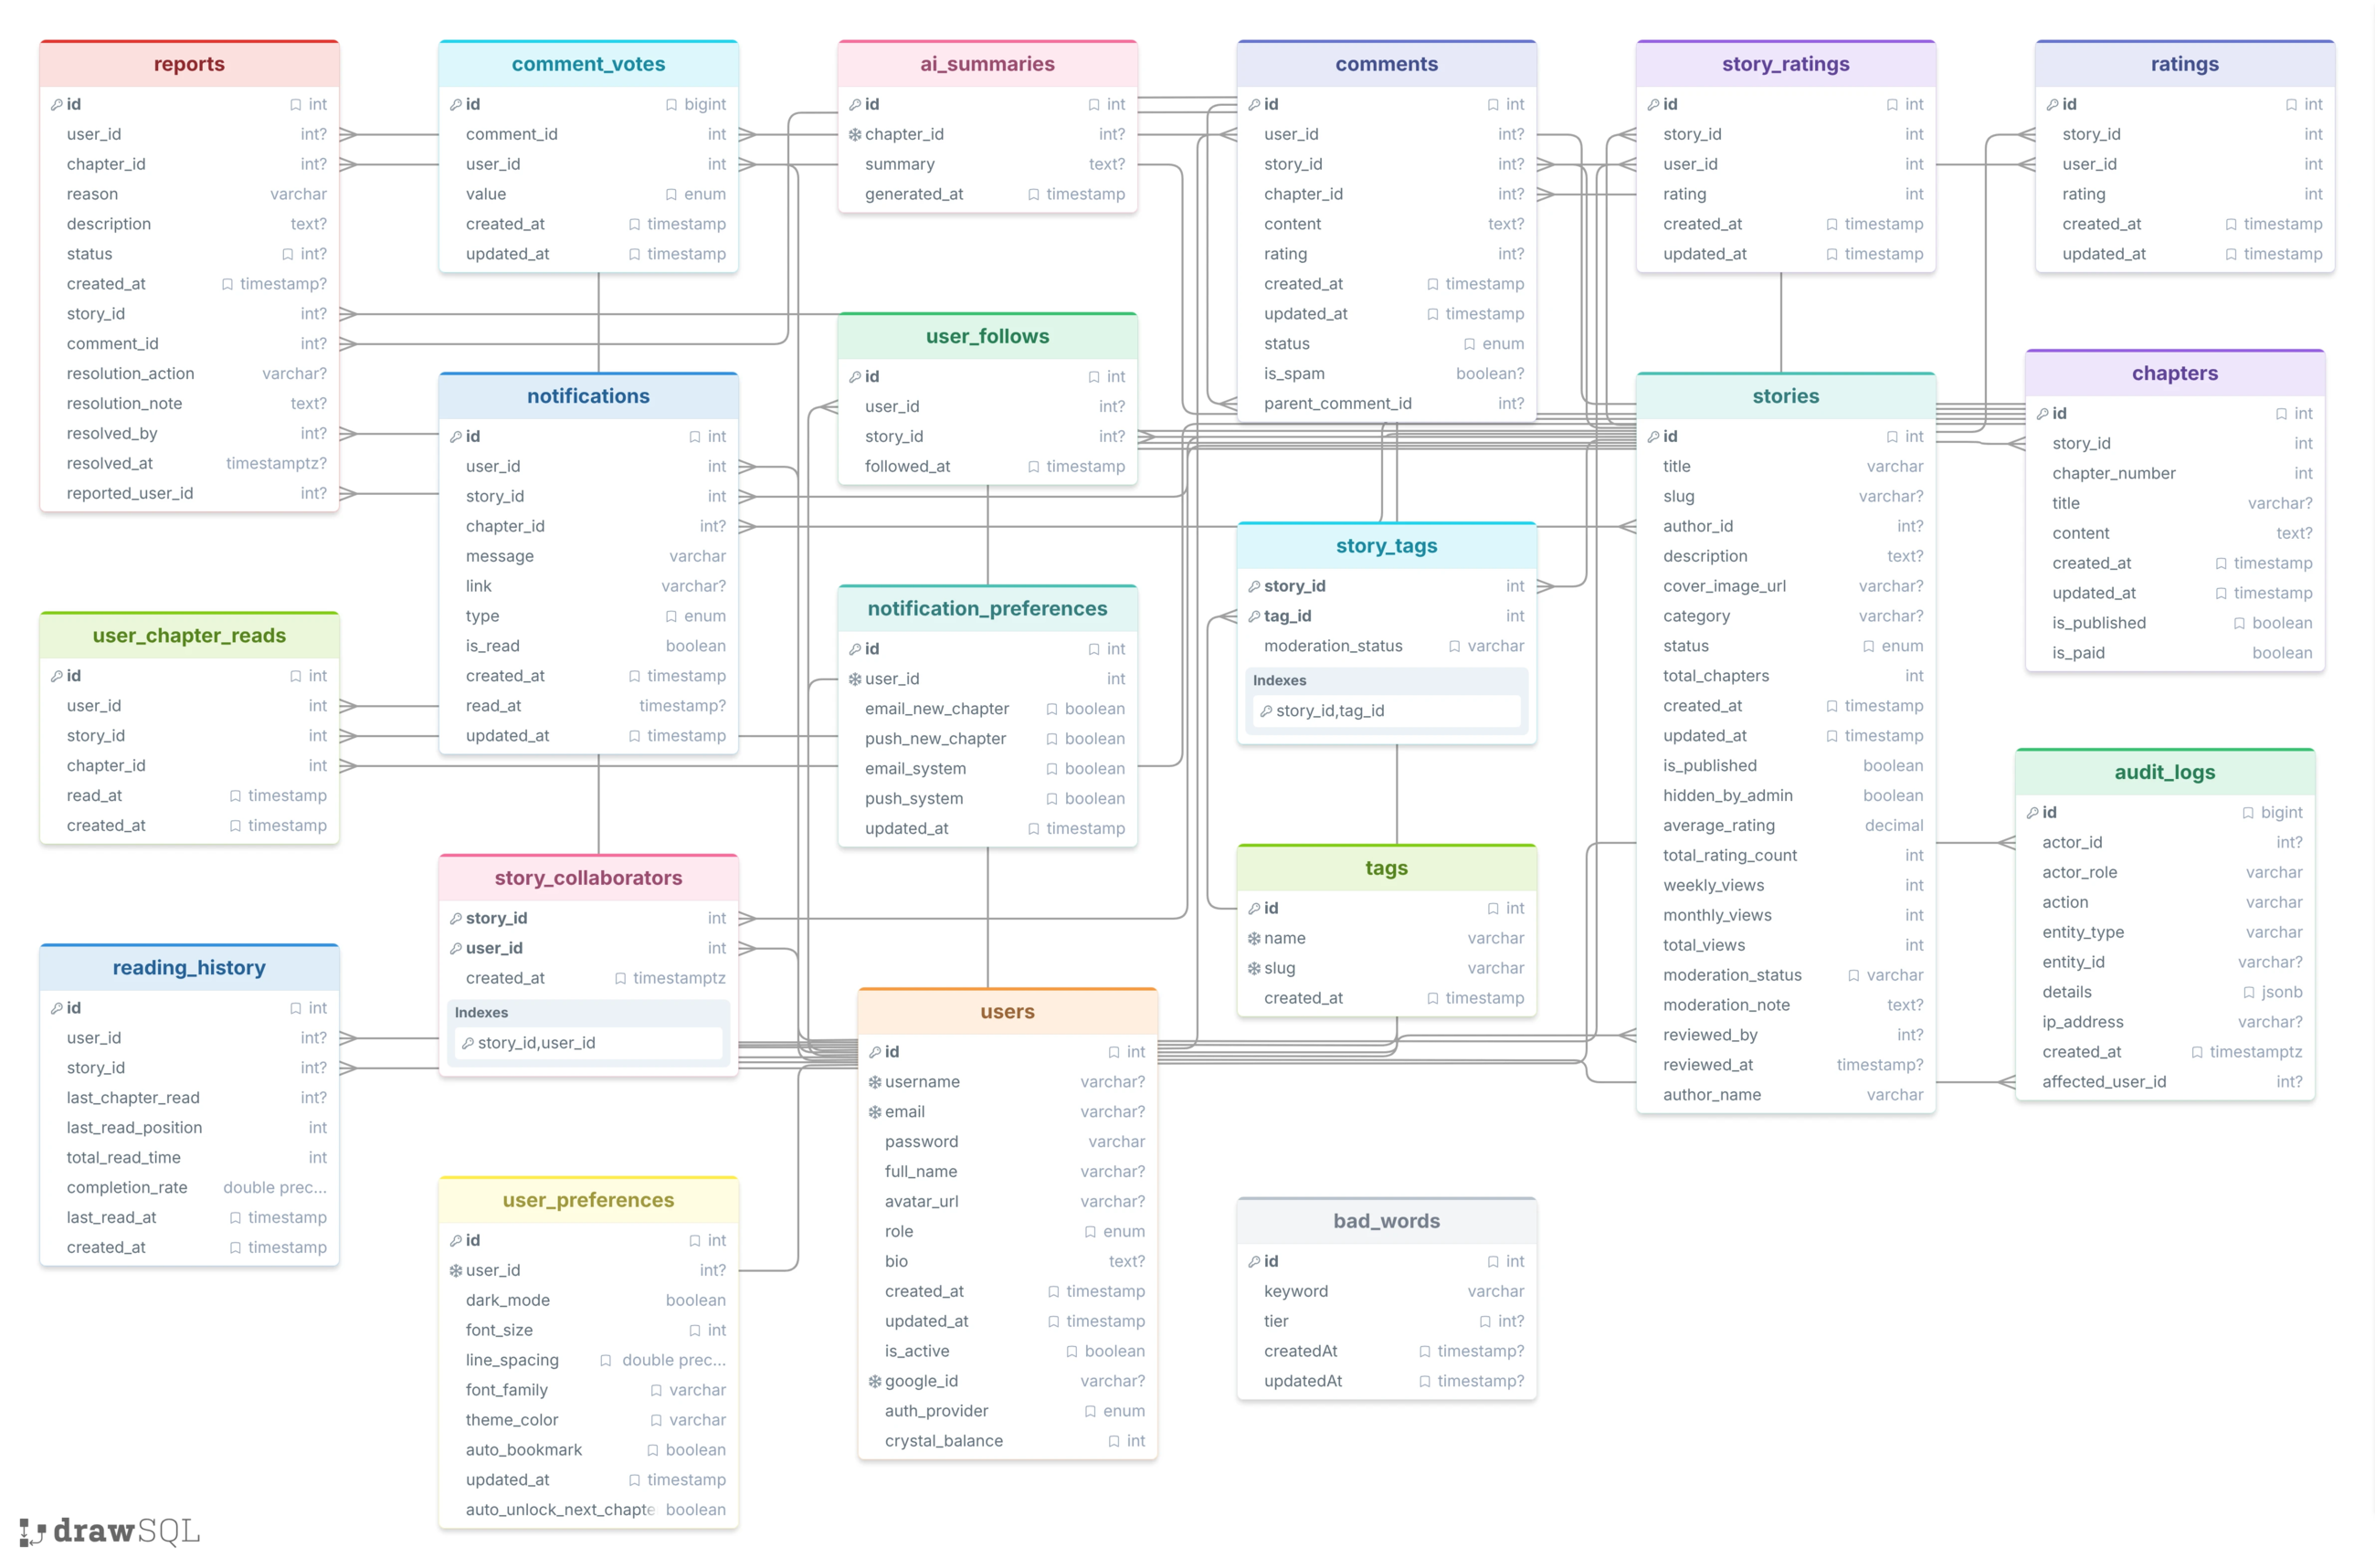
\includegraphics[width=\linewidth,height=0.85\textheight,keepaspectratio]{images/database-erd.png}
  \captionof{figure}{Lược đồ ERD của cơ sở dữ liệu CMC Truyện\label{fig:database-er}}
\end{center}
\vspace*{\fill}
\end{landscape}

Hình~\ref{fig:database-er} thể hiện các quan hệ chính của hệ thống. \CodePath{users}, \CodePath{stories} và \CodePath{chapters} là ba thực thể trung tâm; các bảng lịch sử đọc, theo dõi, đánh giá, bình luận và thông báo liên kết hành vi người dùng với nội dung. Nhóm bảng \CodePath{reports}, \CodePath{bad_words} và \CodePath{audit_logs} phục vụ kiểm duyệt và truy vết.


\ReportImage[1.0\textheight]
  {images/screenshots/db-folder-schema.png}
  {Cấu trúc script, migration và schema cơ sở dữ liệu}
  {fig:db-folder}
  {Chụp \CodePath{backend/scripts} và \CodePath{backend/src/scripts/migrations}; hiển thị tên file, không chụp chuỗi kết nối.}

\ReportImage[1.0\textheight]
  {images/screenshots/db-main-sql-code.png}
  {Đoạn SQL chính về bảng truyện, chương và ràng buộc}
  {fig:db-sql-code}
  {Chụp đoạn code thật trong \CodePath{schema.sql}, ưu tiên primary key, foreign key, CHECK, UNIQUE và index.}

\clearpage
\subsection{Connection pool, index và transaction}

Backend cấu hình PostgreSQL Pool với tối đa 20 connection, idle timeout 30 giây và connection timeout 5 giây. Môi trường production có thể dùng \CodePath{DATABASE_URL}; môi trường local có thể dùng các biến host/port/name/user/password. Index tập trung vào slug, danh sách truyện công khai, số chương, trạng thái bình luận, khóa ngoại và audit. API danh sách chương không trả trường content, qua đó giảm kích thước phản hồi.

Khi một nghiệp vụ có nhiều bước ghi dữ liệu, tất cả query từ \CodePath{BEGIN} đến \CodePath{COMMIT/ROLLBACK} phải dùng cùng client lấy từ \CodePath{pool.connect()}. Nếu trộn \CodePath{pool.query()} với client trong một transaction, các query có thể chạy trên connection khác và rollback không còn bảo đảm tính nguyên tử.
Nghiệp vụ mở khóa chương là ví dụ điển hình cho transaction nhiều bước. Model \CodePath{Wallet.unlockChapter} khóa bản ghi số dư của người dùng bằng \CodePath{FOR UPDATE}, kiểm tra bản ghi mở khóa hiện có và số dư trước khi ghi dữ liệu. Nếu bất kỳ bước nào thất bại, \CodePath{ROLLBACK} bảo đảm số dư, lịch sử giao dịch và quyền đọc không rơi vào trạng thái không nhất quán.



\section{Cấu hình và triển khai}

\subsection{Biến môi trường}

Các biến chính gồm URL frontend/backend, PostgreSQL, Redis, JWT, Google OAuth, Resend, Supabase và nhà cung cấp AI. File \CodePath{.env} không được commit. Frontend chỉ nhận biến public như \CodePath{VITE_API_URL}; service key, JWT secret và AI key phải ở backend.

\begin{table}[htbp]
\centering
\caption{Nhóm biến môi trường và nguyên tắc bảo mật}
\label{tab:environment-vars}
\begin{tabularx}{\textwidth}{|>{\bfseries\RaggedRight\arraybackslash}p{3.2cm}|X|X|}
\hline
\textbf{Nhóm} & \textbf{Ví dụ tên biến} & \textbf{Nguyên tắc} \\
\hline
Database & DATABASE\_URL, DB\_HOST, DB\_NAME & Chỉ backend; production ưu tiên secret manager. \\
\hline
Auth & JWT\_SECRET, GOOGLE\_CLIENT\_ID & Secret đủ mạnh; không dùng fallback production. \\
\hline
Queue & REDIS\_URL & API và worker dùng cùng instance; bật TLS nếu nhà cung cấp yêu cầu. \\
\hline
Email/Storage & RESEND\_API\_KEY, SUPABASE\_SERVICE\_KEY & Service key không xuất hiện trong bundle frontend/log. \\
\hline
AI & GROQ\_API\_KEY, GEMINI\_API\_KEY & Chỉ backend; đặt timeout, quota và theo dõi lỗi. \\
\hline
Frontend & VITE\_API\_URL & Có thể công khai; trỏ đúng tiền tố \CodePath{/\allowbreak{}api}. \\
\hline
\end{tabularx}
\end{table}

\subsection{Topology triển khai}

\CodePath{Render.yaml} khai báo hai service Node: web service chạy backend và worker chạy \CodePath{src/startWorker.js}. Frontend có \CodePath{vercel.json} rewrite mọi route SPA về \CodePath{index.html}. PostgreSQL và Redis không được khai báo trực tiếp trong file Render; chúng phải được cung cấp qua dịch vụ managed hoặc hạ tầng khác và cấu hình bằng environment.

\begin{table}[htbp]
\centering
\caption{Liên kết bàn giao và minh chứng triển khai}
\label{tab:delivery-links}
\begin{tabularx}{\textwidth}{|>{\bfseries\RaggedRight\arraybackslash}p{4.0cm}|X|}
\hline
\textbf{Hạng mục} & \textbf{Liên kết} \\
\hline
Website chạy thực tế & \OptionalURL{\WebsiteURL}{https://thanhnt2k.app/} \\
\hline
Kho source dùng để nộp & \OptionalURL{\SourceCodeURL}{https://github.com/suzynotsusie/cmc-truyen-temp} \\
\hline
\end{tabularx}
\end{table}

\clearpage

\section{Kiểm thử và kết quả xác minh}

\subsection{Chiến lược kiểm thử}

Dự án áp dụng chiến lược kiểm thử theo mô hình tháp (Testing Pyramid) với ba tầng chính: unit/integration test chiếm phần lớn (Jest cho backend, Vitest và Testing Library cho frontend), E2E test tự động bằng Playwright cho các luồng nghiệp vụ quan trọng, và kiểm thử thủ công bổ sung cho kịch bản khó tự động hóa. Toàn bộ dependency ngoài (database, Redis, Supabase, email) được mock trong bộ test mặc định để đảm bảo CI ổn định; kiểm thử với hạ tầng thật được lên kế hoạch trên môi trường staging riêng. Bảng~\ref{tab:test-tools} tóm tắt công cụ theo từng tầng.

\begin{table}[htbp]
\centering
\caption{Công cụ và phạm vi kiểm thử theo tầng}
\label{tab:test-tools}
\begin{tabularx}{\textwidth}{|>{\RaggedRight\arraybackslash}p{3.2cm}|>{\RaggedRight\arraybackslash}p{4.0cm}|X|}
\hline
\textbf{Tầng kiểm thử} & \textbf{Công cụ} & \textbf{Phạm vi} \\
\hline
Unit / Integration & Jest, Supertest & Backend: controller, service, middleware, RBAC, audit \\
\hline
Component / Unit & Vitest, Testing Library & Frontend: component, hook, route guard, UI behavior \\
\hline
End-to-End & Playwright & Luồng đăng nhập, tìm kiếm và đọc truyện \\
\hline
Performance & Jest (budget test) & Parse 1.000 chương trong ngân sách thời gian định nghĩa \\
\hline
Thủ công & Trình duyệt, DevTools & Responsive, edge case UX, luồng phân quyền phức tạp \\
\hline
\end{tabularx}
\end{table}

\subsection{Kết quả tổng hợp}

Bộ test mặc định và build frontend được chạy trực tiếp trên workspace dự án. Kết quả được ghi ở Bảng~\ref{tab:test-results}; đây là số liệu của lần chạy thực tế, không phải con số giả định.

\begin{table}[H]
\centering
\caption{Kết quả kiểm thử và build đã thực chạy}
\label{tab:test-results}
\begin{tabularx}{\textwidth}{|>{\RaggedRight\arraybackslash}p{4.0cm}|>{\centering\arraybackslash}p{2.5cm}|X|}
\hline
\textbf{Hạng mục} & \textbf{Kết quả} & \textbf{Ghi chú quan sát} \\
\hline
Backend (Jest) & 121/121 pass & 21 test suite pass; có log Redis \CodePath{ECONNREFUSED} và Jest force-exit do \CodePath{BullMQ} queue chưa đóng sau test. \\
\hline
Frontend (Vitest) & 36/36 pass & 11 test file pass; có cảnh báo tùy chọn \CodePath{esbuild}/\CodePath{oxc} deprecated từ toolchain. \\
\hline
Tổng test mặc định & 157/157 pass & Lệnh root test hoàn thành exit code 0. \\
\hline
Frontend production build & Thành công & 209 module transformed; build trong 2,13 giây; cảnh báo dynamic import cho \CodePath{mockStories.js}. \\
\hline
Bundle JavaScript & 641,96 kB & Gzip 192,47 kB; Vite cảnh báo chunk lớn hơn 500 kB. \\
\hline
E2E Playwright & 6/6 pass & 100\% pass (6 kịch bản: login reader, login sai, mất mạng, login admin, tìm kiếm, đọc chương). \\
\hline
Performance (parse 1.000 chương) & Đạt ngân sách & Service parse tệp hoàn thành dưới ngưỡng thời gian định nghĩa trong \CodePath{storyFileImportService.\allowbreak{}performance.\allowbreak{}test.js}. \\
\hline
\end{tabularx}
\end{table}

Các bài kiểm thử đều đã vượt qua thành công, chứng minh các vùng logic cốt lõi đã được bảo vệ đầy đủ: từ health, auth, RBAC, audit, OTP, đến import file, ranking, kiểm duyệt, báo cáo và luồng xử lý truyện. Lỗi kết nối Redis \CodePath{ECONNREFUSED} xuất hiện trong log là bình thường khi chạy ở môi trường local không có sẵn service Redis. Về việc Jest bị force-exit, nguyên nhân xuất phát từ việc hàng đợi \CodePath{BullMQ} chưa được đóng đúng cách trong \CodePath{afterAll}. Để khắc phục triệt để, chúng ta cần bổ sung logic teardown nhằm giải phóng kết nối, đồng thời tích hợp \CodePath{ioredis-mock} để cô lập hoàn toàn các unit test. Cuối cùng, kích thước bundle JavaScript hiện đạt 641,96~kB, vượt quá giới hạn khuyến nghị 500~kB của Vite. Giải pháp cần triển khai là áp dụng route-level lazy loading kết hợp chia nhỏ vendor chunk, sau đó đo đạc lại để kiểm chứng.
\clearpage

\subsection{Nhóm 1: Xác thực người dùng}

Kết quả kiểm thử tự động cho luồng xác thực người dùng (đăng nhập, đăng ký, quên mật khẩu và xác thực OTP) được tổng hợp tại Bảng~\ref{tab:tc-auth}. Quá trình kiểm thử bao gồm 18 kịch bản, được thực thi qua các test suite: \CodePath{authController.login.test.js}, \CodePath{authController.account.test.js} và \CodePath{otpService.test.js}, nhằm đảm bảo tính bảo mật và trải nghiệm xuyên suốt của hệ thống.

\begingroup
\footnotesize
\begin{longtable}{|>{\centering\arraybackslash}p{0.5cm}|>{\RaggedRight\arraybackslash}p{2.0cm}|>{\RaggedRight\arraybackslash}p{3.5cm}|>{\RaggedRight\arraybackslash}p{2.2cm}|>{\RaggedRight\arraybackslash}p{2.2cm}|>{\RaggedRight\arraybackslash}p{3.1cm}|}
\caption{Test case nhóm xác thực người dùng}\label{tab:tc-auth}\\
\hline
\textbf{STT} & \textbf{Test Case} & \textbf{Input} & \textbf{Output} & \textbf{Kết quả mong muốn} & \textbf{Kết quả thực tế} \\
\hline
\endfirsthead
\hline
\textbf{STT} & \textbf{Test Case} & \textbf{Input} & \textbf{Output} & \textbf{Kết quả mong muốn} & \textbf{Kết quả thực tế} \\
\hline
\endhead
\hline
\multicolumn{6}{|r|}{\emph{Còn tiếp ở trang sau}}\\
\hline
\endfoot
\hline
\endlastfoot
1 & Đăng nhập đúng tài khoản & Email \texttt{reader\allowbreak{}@\allowbreak{}example.\allowbreak{}com}, password \texttt{Password1!} & HTTP \texttt{200}, JWT và user & Đăng nhập thành công; response không chứa password & HTTP \texttt{200}, có token, password đã bị loại bỏ (\textbf{Đạt}) \\
\hline
2 & Đúng email, sai mật khẩu & Email hợp lệ, password \texttt{WrongPassword1!} & HTTP \texttt{401}, thông báo tiếng Việt & Không cấp token & HTTP \texttt{401}, UI hiển thị thông báo tiếng Việt (\textbf{Đạt}) \\
\hline
3 & Sai email, đúng mật khẩu của tài khoản khác & Email \texttt{unknown\allowbreak{}@\allowbreak{}example.\allowbreak{}com}, password hợp lệ & HTTP \texttt{401}, cùng thông báo lỗi & Không đăng nhập và không tiết lộ email tồn tại hay không & HTTP \texttt{401}, cùng thông báo tiếng Việt (\textbf{Đạt}) \\
\hline
4 & Email đăng nhập sai định dạng & \texttt{reader-at-\allowbreak{}example.\allowbreak{}com} & HTTP \texttt{400}, lỗi định dạng & Chặn trước khi truy vấn database & HTTP \texttt{400}, lỗi hiển thị bằng tiếng Việt (\textbf{Đạt}) \\
\hline
5 & Email dùng ký tự Unicode full-width & Chuỗi email toàn ký tự full-width & HTTP \texttt{400}, dữ liệu không hợp lệ & Không chấp nhận định dạng ký tự sai & HTTP \texttt{400}, không truy vấn user (\textbf{Đạt}) \\
\hline
6 & Database lỗi khi đăng nhập & Credentials hợp lệ; DB không khả dụng & HTTP \texttt{500}, thông báo chung & Không cấp token và không lộ lỗi nội bộ & HTTP \texttt{500}, thông báo chung bằng tiếng Việt (\textbf{Đạt}) \\
\hline
7 & Đăng ký hợp lệ & Username \texttt{Reader\_01}, email hợp lệ, password mạnh & HTTP \texttt{201}, token và role \texttt{User} & Tạo tài khoản, hash password, không trả hash & Role \texttt{User}, response không có password (\textbf{Đạt}) \\
\hline
8 & Username đã tồn tại & Username trùng tài khoản hiện có & HTTP \texttt{409} & Không kiểm tra/tạo tiếp bằng email & HTTP \texttt{409}, không gọi tạo user (\textbf{Đạt}) \\
\hline
9 & Email đã tồn tại & Username mới, email trùng & HTTP \texttt{409} & Không tạo tài khoản trùng & HTTP \texttt{409}, không gọi tạo user (\textbf{Đạt}) \\
\hline
10 & Username sai định dạng & Username có dấu hoặc khoảng trắng & HTTP \texttt{400} & Chỉ nhận chữ không dấu, số, \texttt{\_}, \texttt{-} & HTTP \texttt{400}, thông báo tiếng Việt (\textbf{Đạt}) \\
\hline
11 & Mật khẩu đăng ký yếu & \texttt{password} (thiếu chữ hoa, số, ký tự đặc biệt) & HTTP \texttt{400}, thông báo tiêu chí & Yêu cầu tối thiểu 8 ký tự, chữ hoa, số và ký tự đặc biệt & HTTP \texttt{400}, không tạo user (\textbf{Đạt}) \\
\hline
12 & Chèn role qua request đăng ký & Payload có thêm \texttt{role: Admin} và \texttt{is\_\allowbreak{}active: false} & User tạo với role \texttt{User} & Chống mass assignment & Field lạ bị loại bỏ, role vẫn là \texttt{User} (\textbf{Đạt}) \\
\hline
13 & Quên mật khẩu với email tồn tại/không tồn tại & Hai email có trạng thái khác nhau & Cùng HTTP \texttt{200} và cùng message & Chống dò tìm email tài khoản & Hai response giống nhau (\textbf{Đạt}) \\
\hline
14 & OTP sai hoặc hết hạn & OTP \texttt{000000} không hợp lệ & HTTP \texttt{400} & Không cho reset password & HTTP \texttt{400}, không cập nhật password (\textbf{Đạt}) \\
\hline
15 & Reset khi chưa xác thực OTP & Password mới hợp lệ nhưng OTP chưa verified & HTTP \texttt{403} & Bắt buộc xác thực OTP trước & HTTP \texttt{403}, không cập nhật password (\textbf{Đạt}) \\
\hline
16 & Reset password thành công & OTP verified; password mạnh và xác nhận khớp & HTTP \texttt{200} & Hash password mới và xóa OTP đã dùng & Password được cập nhật, OTP keys được xóa (\textbf{Đạt}) \\
\hline
17 & Gửi form login hai lần (double-click) & Double-click nút đăng nhập khi request đang xử lý & Chỉ một request; nút bị disabled & Không tạo request đăng nhập trùng & Hàm login chỉ được gọi một lần (\textbf{Đạt}) \\
\hline
18 & Mất mạng khi đăng nhập & API login bị ngắt kết nối & UI giữ nguyên \texttt{/\allowbreak{}login} và hiện lỗi & Cho phép người dùng thử lại, không crash & Alert lỗi hiển thị, không chuyển trang (\textbf{Đạt}) \\
\hline
\end{longtable}
\endgroup

\clearpage

\subsection{Nhóm 2: Upload truyện và kiểm duyệt}

Quy trình đăng tải truyện và các bước kiểm duyệt được đánh giá qua 21 kịch bản kiểm thử tự động (Bảng~\ref{tab:tc-upload}). Quá trình này xác minh các ràng buộc về quyền sở hữu, giới hạn kích thước tệp tải lên (tối đa 25~MB) và luồng công việc xét duyệt của Moderator. Các test suite đảm nhiệm bao gồm: \CodePath{uploadStoryFile.test.js}, \CodePath{chapterController.upload.test.js}, \CodePath{storyWorkflow.test.js} và \CodePath{moderatorController.test.js}.

\begingroup
\footnotesize
\begin{longtable}{|>{\centering\arraybackslash}p{0.5cm}|>{\RaggedRight\arraybackslash}p{2.0cm}|>{\RaggedRight\arraybackslash}p{3.5cm}|>{\RaggedRight\arraybackslash}p{2.2cm}|>{\RaggedRight\arraybackslash}p{2.2cm}|>{\RaggedRight\arraybackslash}p{3.1cm}|}
\caption{Test case nhóm upload truyện và kiểm duyệt}\label{tab:tc-upload}\\
\hline
\textbf{STT} & \textbf{Test Case} & \textbf{Input} & \textbf{Output} & \textbf{Kết quả mong muốn} & \textbf{Kết quả thực tế} \\
\hline
\endfirsthead
\hline
\textbf{STT} & \textbf{Test Case} & \textbf{Input} & \textbf{Output} & \textbf{Kết quả mong muốn} & \textbf{Kết quả thực tế} \\
\hline
\endhead
\hline
\multicolumn{6}{|r|}{\emph{Còn tiếp ở trang sau}}\\
\hline
\endfoot
\hline
\endlastfoot
1 & Upload TXT UTF-8 vào truyện đã duyệt & Uploader là chủ sở hữu; \texttt{truyen.txt} UTF-8; truyện approved & HTTP \texttt{201},\newline\texttt{imported\_\allowbreak{}count: 1} & Tạo đúng chương và số chương kế tiếp & Tạo 1 chương, \texttt{next\_\allowbreak{}chapter\_\allowbreak{}number: 2} (\textbf{Đạt}) \\
\hline
2 & Upload nội dung UTF-16 LE tiếng Việt & TXT có BOM UTF-16 LE & HTTP \texttt{200} khi preview & Không lỗi font hoặc mất dấu & Tiêu đề/nội dung tiếng Việt giữ nguyên (\textbf{Đạt}) \\
\hline
3 & Không chọn file & Request không có field \texttt{file} & HTTP \texttt{400} & Không tạo chương, báo thiếu file & HTTP \texttt{400}, batch insert không được gọi (\textbf{Đạt}) \\
\hline
4 & File không có nội dung đọc được & TXT chỉ chứa byte NUL & HTTP \texttt{400},\newline\texttt{success: false} & Không import dữ liệu rác & HTTP \texttt{400}, không tạo chương (\textbf{Đạt}) \\
\hline
5 & Sai đuôi file & \texttt{truyen.exe} & HTTP \texttt{400} & Chỉ chấp nhận \texttt{.txt}, \texttt{.md}, \texttt{.epub} & Middleware từ chối file (\textbf{Đạt}) \\
\hline
6 & Đuôi đúng nhưng MIME sai & \texttt{truyen.txt}, MIME \texttt{image/\allowbreak{}png} & HTTP \texttt{400} & Kiểm tra cả extension và MIME type & Middleware trả lỗi định dạng (\textbf{Đạt}) \\
\hline
7 & File vượt kích thước 25~MB & TXT lớn hơn 25~MB & HTTP \texttt{400},\newline\texttt{LIMIT\_\allowbreak{}FILE\_\allowbreak{}SIZE} & Chặn file quá giới hạn & Nhận đúng mã\newline\texttt{LIMIT\_\allowbreak{}FILE\_\allowbreak{}SIZE} (\textbf{Đạt}) \\
\hline
8 & Chưa đăng nhập khi import & Không có \texttt{req.user} & HTTP \texttt{401} & Yêu cầu xác thực & HTTP \texttt{401}, không truy vấn truyện (\textbf{Đạt}) \\
\hline
9 & Uploader không sở hữu truyện & User \texttt{99} import vào truyện của user \texttt{7} & HTTP \texttt{403} & Chỉ owner/\allowbreak{}collaborator/\allowbreak{}Admin được thao tác & HTTP \texttt{403}, không tạo chương (\textbf{Đạt}) \\
\hline
10 & Import khi truyện chưa duyệt & Truyện \texttt{pending}, chưa publish & HTTP \texttt{409} & Chỉ import sau khi Moderator duyệt & HTTP \texttt{409}, không tạo chương (\textbf{Đạt}) \\
\hline
11 & Database lỗi khi import & File hợp lệ; DB không khả dụng & HTTP \texttt{500},\newline\texttt{success: false} & Không trả số chương thành công giả & HTTP \texttt{500}, không trả success (\textbf{Đạt}) \\
\hline
12 & Tạo truyện mới & Metadata hợp lệ từ Uploader & HTTP \texttt{201}; truyện chờ duyệt & Lưu uploader và tên tác giả riêng biệt & \texttt{author\_\allowbreak{}id} và \texttt{author\_\allowbreak{}name} lưu đúng (\textbf{Đạt}) \\
\hline
13 & Thêm chương trước khi truyện được duyệt & Truyện \texttt{pending} & HTTP \texttt{409} & Không cho thêm chương & HTTP \texttt{409}, model tạo chương không được gọi (\textbf{Đạt}) \\
\hline
14 & Số chương bị trùng & Chapter number đã tồn tại & HTTP \texttt{409},\newline\texttt{CHAPTER\_\allowbreak{}NUMBER\_\allowbreak{}EXISTS} & Không trả lỗi máy chủ chung chung & HTTP \texttt{409}, đúng mã nghiệp vụ (\textbf{Đạt}) \\
\hline
15 & Uploader tự publish truyện & Uploader gọi toggle visibility & HTTP \texttt{403} & Xuất bản phải qua Moderator/\allowbreak{}Admin & HTTP \texttt{403}, không cập nhật truyện (\textbf{Đạt}) \\
\hline
16 & Preview file truyện & TXT có heading chương & HTTP \texttt{200}, danh sách preview & Preview không tạo dữ liệu chương & Có preview, \texttt{Chapter.\allowbreak{}createChapter} không được gọi (\textbf{Đạt}) \\
\hline
17 & Moderator duyệt truyện pending & Story đang trong moderation queue & HTTP \texttt{200} & Chuyển trạng thái đúng và publish & Truyện được duyệt theo workflow (\textbf{Đạt}) \\
\hline
18 & Moderator yêu cầu sửa có lý do & Action request changes và reason hợp lệ & HTTP thành công, có notification & Lưu lý do và thông báo Uploader & Trạng thái và notification được cập nhật (\textbf{Đạt}) \\
\hline
19 & Moderator yêu cầu sửa thiếu lý do & Action request changes, reason rỗng & HTTP \texttt{400} & Bắt buộc có lý do & HTTP \texttt{400}, không cập nhật truyện (\textbf{Đạt}) \\
\hline
20 & Moderator lọc danh sách theo tiêu chí & Status/\allowbreak{}search/\allowbreak{}page/\allowbreak{}limit & Danh sách và global status counts & Lọc đúng; count phản ánh toàn hệ thống & Kết quả lọc và counts đúng (\textbf{Đạt}) \\
\hline
21 & Xử lý report avatar & Report avatar gắn với user bị báo cáo & HTTP thành công & Cập nhật đúng boolean/status, không nhầm enum & Tham số cập nhật tách biệt đúng (\textbf{Đạt}) \\
\hline
\end{longtable}
\endgroup

\clearpage

\subsection{Nhóm 3: Chức năng người dùng}

Các tính năng tương tác của người dùng như tìm kiếm, theo dõi truyện, bình luận, đánh giá, báo cáo vi phạm, tải ảnh đại diện và mở khóa chương bằng Tinh thạch được kiểm chứng thông qua 29 kịch bản (Bảng~\ref{tab:tc-user}). Việc kiểm thử được thực hiện qua các test suite: \CodePath{socialInteractions.test.js}, \CodePath{storyDiscoveryRating.test.js}, \CodePath{reportController.test.js}, \CodePath{chapterUnlock.test.js} và \CodePath{uploadCover.test.js}.

\begingroup
\footnotesize
\begin{longtable}{|>{\centering\arraybackslash}p{0.5cm}|>{\RaggedRight\arraybackslash}p{2.0cm}|>{\RaggedRight\arraybackslash}p{3.5cm}|>{\RaggedRight\arraybackslash}p{2.2cm}|>{\RaggedRight\arraybackslash}p{2.2cm}|>{\RaggedRight\arraybackslash}p{3.1cm}|}
\caption{Test case nhóm chức năng người dùng}\label{tab:tc-user}\\
\hline
\textbf{STT} & \textbf{Test Case} & \textbf{Input} & \textbf{Output} & \textbf{Kết quả mong muốn} & \textbf{Kết quả thực tế} \\
\hline
\endfirsthead
\hline
\textbf{STT} & \textbf{Test Case} & \textbf{Input} & \textbf{Output} & \textbf{Kết quả mong muốn} & \textbf{Kết quả thực tế} \\
\hline
\endhead
\hline
\multicolumn{6}{|r|}{\emph{Còn tiếp ở trang sau}}\\
\hline
\endfoot
\hline
\endlastfoot
1 & Upload avatar JPG/\allowbreak{}PNG/\allowbreak{}WebP hợp lệ & File nhỏ hơn hoặc bằng 5~MB, MIME ảnh & HTTP \texttt{200} qua middleware & Chấp nhận các ảnh hợp lệ & Cả JPG, PNG, WebP đều được nhận (\textbf{Đạt}) \\
\hline
2 & Upload file script giả avatar & \texttt{..\allowbreak{}/\allowbreak{}attack.svg}, MIME \texttt{text/\allowbreak{}html} & HTTP \texttt{400} & Không nhận nội dung không phải ảnh & Middleware từ chối (\textbf{Đạt}) \\
\hline
3 & Avatar vượt 5~MB & PNG lớn hơn 5~MB & HTTP \texttt{400},\newline\texttt{LIMIT\_\allowbreak{}FILE\_\allowbreak{}SIZE} & Chặn file quá lớn & Nhận đúng mã giới hạn (\textbf{Đạt}) \\
\hline
4 & Tìm kiếm kết hợp & Query có dấu/ký tự đặc biệt, category, tag, page & HTTP \texttt{200}, stories và pagination & Truyền đúng bộ lọc, không crash & Model nhận đúng tham số, HTTP \texttt{200} (\textbf{Đạt}) \\
\hline
5 & Tìm kiếm không có kết quả & Từ khóa không tồn tại & HTTP \texttt{200},\newline\texttt{stories: []} & Danh sách rỗng không phải lỗi & HTTP \texttt{200}, mảng rỗng (\textbf{Đạt}) \\
\hline
6 & Guest xem truyện nháp & Slug của truyện chưa publish & HTTP \texttt{404} & Không lộ nội dung chưa duyệt & HTTP \texttt{404} (\textbf{Đạt}) \\
\hline
7 & Guest kiểm tra trạng thái follow & Không có user/token & HTTP \texttt{200},\newline\texttt{following: false} & Endpoint optional auth không trả \texttt{401} & HTTP \texttt{200}, \texttt{false} (\textbf{Đạt}) \\
\hline
8 & Follow/unfollow lặp lại & Gọi follow hai lần, unfollow hai lần & Các request thành công/idempotent & Không gây lỗi hoặc dữ liệu trùng & Controller xử lý các lần gọi ổn định (\textbf{Đạt}) \\
\hline
9 & Follow với story ID sai & ID \texttt{0}, \texttt{-1}, \texttt{abc} & HTTP \texttt{400} & Chỉ nhận ID nguyên dương & Cả ba trường hợp đều bị từ chối (\textbf{Đạt}) \\
\hline
10 & Follow API thất bại, UI tự động rollback & UI cập nhật trước (optimistic); API reject & UI rollback trạng thái & Không để trạng thái giả trên giao diện & Nút follow quay lại trạng thái trước (\textbf{Đạt}) \\
\hline
11 & Bình luận rỗng hoặc quá dài & Khoảng trắng hoặc hơn 2.000 ký tự & HTTP \texttt{400} & Không tạo bình luận sai & HTTP \texttt{400}, model create không được gọi (\textbf{Đạt}) \\
\hline
12 & Reply sang thread khác & Parent thuộc story/\allowbreak{}chapter khác & HTTP \texttt{400} & Không gắn reply sai thread & HTTP \texttt{400}, không tạo comment (\textbf{Đạt}) \\
\hline
13 & User xóa bình luận của người khác & User thường không phải owner & HTTP \texttt{403} & Bảo vệ quyền sở hữu comment & HTTP \texttt{403}, không xóa (\textbf{Đạt}) \\
\hline
14 & Admin xóa bình luận bất kỳ & Admin xóa comment của user khác & HTTP \texttt{200} & Admin được phép moderation & Comment được xóa (\textbf{Đạt}) \\
\hline
15 & Vote sai giá trị & Vote \texttt{0}, \texttt{2}, \texttt{-2} & HTTP \texttt{400} & Chỉ nhận \texttt{1} hoặc \texttt{-1} & Cả ba giá trị bị từ chối (\textbf{Đạt}) \\
\hline
16 & Rating ngoài khoảng hợp lệ & Rating \texttt{0}, \texttt{6}, \texttt{1.5}, \texttt{"five"} & HTTP \texttt{400} & Chỉ nhận số nguyên 1--5 & Không gọi upsert rating (\textbf{Đạt}) \\
\hline
17 & Thêm/cập nhật rating hợp lệ & Rating \texttt{5} của user đăng nhập & HTTP \texttt{200}, summary mới & Upsert rating của đúng user & Model nhận story ID, user ID và rating đúng (\textbf{Đạt}) \\
\hline
18 & Xóa rating của chính user & User xóa rating của mình & HTTP \texttt{200}, summary mới & Không xóa rating của user khác & Model được gọi với đúng user hiện tại (\textbf{Đạt}) \\
\hline
19 & Tạo report hợp lệ & User, target story, reason, description & HTTP \texttt{201} & Tạo report đúng target & Insert đúng dữ liệu (\textbf{Đạt}) \\
\hline
20 & Spam report vượt rate limit & Đã gửi đủ giới hạn trong một giờ & HTTP \texttt{429} & Chặn spam trước khi insert & HTTP \texttt{429}, không insert report (\textbf{Đạt}) \\
\hline
21 & Report avatar từ comment & Comment ID có tác giả & Report gắn\newline\texttt{reported\_\allowbreak{}user\_\allowbreak{}id} & Moderator biết đúng user bị báo cáo & User ID được lấy từ tác giả comment (\textbf{Đạt}) \\
\hline
22 & Cập nhật report không tồn tại & Report ID không có trong DB & HTTP \texttt{404} & Không tạo trạng thái giả & HTTP \texttt{404} (\textbf{Đạt}) \\
\hline
23 & Hành động report sai loại target & Dùng chapter action cho comment report & HTTP \texttt{400} & Chặn action không tương thích & HTTP \texttt{400}, không cập nhật target (\textbf{Đạt}) \\
\hline
24 & Mở khóa chương miễn phí & Chapter \texttt{is\_\allowbreak{}paid: false} & HTTP \texttt{409}, không trừ tiền & Không gọi giao dịch ví & Wallet không được gọi (\textbf{Đạt}) \\
\hline
25 & Mở khóa chương trả phí & Chapter khóa; số dư đủ & HTTP \texttt{200},\newline\texttt{CHAPTER\_\allowbreak{}UNLOCKED} & Trừ đúng \CodePath{UNLOCK_COST} và trả số dư mới & Chương được mở, số dư giảm đúng chi phí cấu hình (\textbf{Đạt}) \\
\hline
26 & Mở khóa lại hoặc request đồng thời & Wallet báo\newline\texttt{already\_\allowbreak{}unlocked: true} & HTTP \texttt{200}, cost \texttt{0} & Không trừ tiền lần hai & \texttt{CHAPTER\_\allowbreak{}ALREADY\_\allowbreak{}UNLOCKED}, cost \texttt{0} (\textbf{Đạt}) \\
\hline
27 & Số dư không đủ khi mở khóa & Balance nhỏ hơn \CodePath{UNLOCK_COST} & HTTP \texttt{409},\newline\texttt{INS\allowbreak{}UFFICI\allowbreak{}ENT\_\allowbreak{}CRYSTALS} & Không mở khóa; trả số dư hiện tại & API trả \texttt{409}, số dư không thay đổi (\textbf{Đạt}) \\
\hline
28 & Database lỗi khi mở khóa & DB error chứa dữ liệu nội bộ & HTTP \texttt{500}, thông báo chung & Không lộ chi tiết database & UI chỉ hiển thị thông báo chung tiếng Việt (\textbf{Đạt}) \\
\hline
\end{longtable}
\endgroup

\clearpage

\subsection{Kiểm thử thủ công bổ sung}

Đối với các nghiệp vụ phức tạp liên quan đến trải nghiệm tương tác giao diện (UI/UX), khả năng hiển thị tương thích đa thiết bị và sự tích hợp với các dịch vụ bên ngoài trong điều kiện thực tế, hệ thống được xác minh bổ sung thông qua phương pháp kiểm thử thủ công. Kết quả đánh giá cho 10 kịch bản đặc thù này được tổng hợp chi tiết tại Bảng~\ref{tab:manual-tests}, qua đó khẳng định hệ thống đáp ứng đầy đủ các yêu cầu đã đặt ra.

\begingroup
\footnotesize
\begin{longtable}{|>{\centering\arraybackslash}p{0.7cm}|>{\RaggedRight\arraybackslash}p{2.0cm}|>{\RaggedRight\arraybackslash}p{3.5cm}|>{\RaggedRight\arraybackslash}p{2.0cm}|>{\RaggedRight\arraybackslash}p{2.2cm}|>{\RaggedRight\arraybackslash}p{3.1cm}|}
\caption{Kịch bản kiểm thử thủ công bổ sung}\label{tab:manual-tests}\\
\hline
\textbf{STT} & \textbf{Test Case} & \textbf{Input} & \textbf{Output} & \textbf{Kết quả mong muốn} & \textbf{Kết quả thực tế} \\
\hline
\endfirsthead
\hline
\textbf{STT} & \textbf{Test Case} & \textbf{Input} & \textbf{Output} & \textbf{Kết quả mong muốn} & \textbf{Kết quả thực tế} \\
\hline
\endhead
\hline
\multicolumn{6}{|r|}{\emph{Còn tiếp ở trang sau}}\\
\hline
\endfoot
\hline
\endlastfoot
MT01 & Xem và đọc truyện public không cần đăng nhập & Guest; có truyện approved; từ khóa tìm kiếm & Trang reader và chi tiết hiển thị bình thường & Không yêu cầu login; URL đúng slug/\allowbreak{}chương & Hiển thị trang reader đầy đủ, URL chứa slug chuẩn (\textbf{Đạt}) \\
\hline
MT02 & Follow truyện và kiểm tra tính nhất quán & User đăng nhập; follow, tải lại, xem danh sách theo dõi & Trạng thái follow đồng bộ DB & Nhất quán với DB; lỗi mạng có rollback & Trạng thái follow/unfollow đồng bộ ngay sau khi tải lại (\textbf{Đạt}) \\
\hline
MT03 & Ghi nhận lịch sử đọc đúng user & User đọc nhiều chương; đọc, cuộn, thoát và mở lịch sử & Lịch sử hiển thị đúng & Trở về đúng truyện/chương; không ghi nhầm user & Lịch sử được lưu đúng tài khoản và vị trí chương đã đọc (\textbf{Đạt}) \\
\hline
MT04 & Uploader không thể thêm chương/publish khi pending & Uploader; truyện pending, chưa duyệt & HTTP \texttt{409}/\texttt{403}, thông báo rõ ràng & Bị chặn với thông báo đúng; không đổi DB & Uploader nhận lỗi HTTP \texttt{409}/\texttt{403} trên cả UI và API (\textbf{Đạt}) \\
\hline
MT05 & Moderator duyệt có/không có lý do & Moderator; truyện pending; lần~1 không nhập lý do, lần~2 nhập lý do & Lần~1: HTTP \texttt{400}; Lần~2: HTTP \texttt{200} & Lần đầu bị validate; lần sau cập nhật trạng thái, notify và audit & Bị chặn khi gửi lý do trống; duyệt thành công khi điền đủ lý do (\textbf{Đạt}) \\
\hline
MT06 & Rate limit khi gửi report nhiều lần & User; gửi report lặp trong 1 giờ & Report đầu: HTTP \texttt{201}; lần sau: HTTP \texttt{429} & Report đầu hợp lệ; request lặp bị hạn chế & API phản hồi HTTP \texttt{429} sau khi gửi report dồn dập (\textbf{Đạt}) \\
\hline
MT07 & Admin thay đổi role/\allowbreak{}status người dùng & Admin đăng nhập; chọn user, đổi role/\allowbreak{}status & UI cập nhật; audit log ghi nhận & UI cập nhật; audit không chứa password/token & Quyền user thay đổi ngay lập tức, audit log ghi nhận đầy đủ (\textbf{Đạt}) \\
\hline
MT08 & Token hết hạn không gây vòng lặp redirect & Token hết hạn; truy cập trang account/\allowbreak{}admin & HTTP \texttt{401}; redirect về \texttt{/\allowbreak{}login} & API trả \texttt{401}; frontend xóa phiên, không lặp vô hạn & API trả \texttt{401}; frontend xóa session và redirect về \texttt{/login} (\textbf{Đạt}) \\
\hline
MT09 & Responsive UI trên mobile và desktop & Viewport 375px và desktop; duyệt Home, Reader, Admin & Layout hiển thị đúng theo viewport & Không tràn ngang; nút thao tác được; chữ đủ đọc & Giao diện hiển thị tốt trên các kích thước màn hình mobile/desktop (\textbf{Đạt}) \\
\hline
MT10 & Queue job notification với Redis thật & Staging với Redis thật; tạo chương mới đủ điều kiện & Job xử lý; notification được tạo & Job xử lý một lần; notification tạo đúng người nhận & Queue job Notification xử lý thành công qua Redis trên staging (\textbf{Đạt}) \\
\hline
\end{longtable}
\endgroup

\section{Kết luận chương}

Chương 3 đã trình bày kiến trúc SPA + REST, thiết kế giao diện theo vai trò, cách tổ chức frontend, backend, cơ sở dữ liệu, triển khai và kiểm thử. Phần đánh giá, hạn chế và hướng hoàn thiện được tổng hợp trong kết luận cuối cùng của báo cáo.

\chapter{CỘNG TÁC TRÊN GITHUB VÀ SỬ DỤNG CÔNG CỤ AI}

\section{Kho mã nguồn và quy ước cộng tác}

Kho mã nguồn công khai được kiểm tra tại \url{https://github.com/suzynotsusie/cmc-truyen-temp}.Hình~\ref{fig:github-repository} là ảnh chụp trực tiếp trang kho mã nguồn dùng làm minh chứng.

\ReportImage[0.35\textheight]
  {images/screenshots/github-repository.png}
  {Kho mã nguồn GitHub của dự án CMC Truyện}
  {fig:github-repository}
  {Ảnh chụp trang GitHub của kho mã nguồn.}

Nhóm làm việc theo vòng lặp: chia nhỏ yêu cầu; tạo nhánh hoặc task; commit theo thay đổi có ý nghĩa; mở pull request khi cần review/tích hợp; chạy test tự động; chỉ đưa commit đạt yêu cầu vào nhánh chính. README là điểm vào cho người mới, trong khi \CodePath{docs/product}, \CodePath{docs/technical}, \CodePath{docs/testing} và \CodePath{docs/ai-logs} lưu bằng chứng chi tiết.

\section{Issues, commits, pull requests, milestones và releases}

\begin{longtable}{|>{\RaggedRight\arraybackslash}p{2.6cm}|>{\RaggedRight\arraybackslash}p{7.0cm}|>{\RaggedRight\arraybackslash}p{5.1cm}|}
\caption{Đối chiếu các cơ chế cộng tác trên GitHub}\label{tab:github-process}\\
\hline
\textbf{Cơ chế} & \textbf{Cách nhóm đã sử dụng / bằng chứng} & \textbf{Đánh giá và hành động đã thực hiện} \\
\hline
\endfirsthead
\hline
\textbf{Cơ chế} & \textbf{Cách nhóm đã sử dụng / bằng chứng} & \textbf{Đánh giá và hành động đã thực hiện} \\
\hline
\endhead
README và tài liệu & README mô tả tính năng, kiến trúc, môi trường, lệnh chạy/test, route và nguyên tắc đóng góp. Product vision, persona, story và backlog nằm trong \CodePath{docs/product/REQUIREMENTS.md}. & Tài liệu đầy đủ, minh bạch và làm điểm mốc thống nhất cho cả dự án. \\
\hline
Commits & Lịch sử có hơn 276 commit trên trang GitHub. Ví dụ: \href{https://github.com/suzynotsusie/cmc-truyen-temp/commit/395f087}{\CodePath{395f087}} (release v1.0.0), \href{https://github.com/suzynotsusie/cmc-truyen-temp/commit/80fdb59}{\CodePath{80fdb59}} (release v1.1.0), \href{https://github.com/suzynotsusie/cmc-truyen-temp/commit/977ccb3}{\CodePath{977ccb3}} (release v1.2.0), \href{https://github.com/suzynotsusie/cmc-truyen-temp/commit/ab78216}{\CodePath{ab78216}} (release v2.0.0). & Có khả năng truy vết thay đổi minh bạch theo từng mốc phát triển. \\
\hline
Pull requests & 13 PR đã đóng, 0 PR mở. PR \href{https://github.com/suzynotsusie/cmc-truyen-temp/pull/12}{\#12} sửa auth/API production; PR \href{https://github.com/suzynotsusie/cmc-truyen-temp/pull/13}{\#13} tự động hóa deploy; các PR \href{https://github.com/suzynotsusie/cmc-truyen-temp/pull/7}{\#7}, \href{https://github.com/suzynotsusie/cmc-truyen-temp/pull/9}{\#9}, \href{https://github.com/suzynotsusie/cmc-truyen-temp/pull/10}{\#10} liên quan đến test và code review. & PR cung cấp điểm review và tích hợp chặt chẽ. Đóng PR không đạt đảm bảo chất lượng nhánh chính. \\
\hline
Issues & Hệ thống đã quản lý đầy đủ 18 GitHub Issues từ \href{https://github.com/suzynotsusie/cmc-truyen-temp/issues/26}{\#26} đến \href{https://github.com/suzynotsusie/cmc-truyen-temp/issues/43}{\#43}, gắn nhãn (labels), phân công công việc (assignees) và liên kết chặt chẽ với các Milestones và PR. & Đạt chuẩn tiêu chí quản lý task minh bạch trên GitHub. \\
\hline
Milestones & Nhóm xây dựng 4 Milestones chính: (1) Core Reading Platform (Issues \#26--\#30, \#32); (2) Engagement \& Search (Issues \#31, \#33--\#36); (3) Moderation \& Safety (Issues \#37--\#40); (4) AI \& Analytics (Issues \#41--\#43). & Quản lý phạm vi phát triển dự án theo đúng quy trình agile/scrum. \\
\hline
Releases & Đã đóng gói 4 phiên bản chính thức trên GitHub: \textbf{v1.0.0} (commit \CodePath{395f087}), \textbf{v1.1.0} (commit \CodePath{80fdb59}), \textbf{v1.2.0} (commit \CodePath{977ccb3}) và \textbf{v2.0.0} (commit \CodePath{ab78216}) với Release Notes chi tiết. & Truy vết phiên bản hệ thống hoàn chỉnh và chuyên nghiệp. \\
\hline
\end{longtable}

Quy trình quản lý trên GitHub được nhóm thực hiện đồng bộ từ việc tạo Issues, gom nhóm vào các Milestones tương ứng, phát triển theo nhánh và kiểm thử tự động, tới việc tạo Tags và Releases đánh dấu mốc hoàn thiện sản phẩm. Dữ liệu đối chiếu hoàn toàn trùng khớp với lịch sử kho mã nguồn.

\section{Code review, kiểm thử tự động và DevOps}

Workflow \CodePath{.github/workflows/tests.yml} chạy khi push, pull request hoặc kích hoạt thủ công, gồm backend Jest, frontend Vitest/build và Playwright E2E. Workflow \CodePath{deploy-production.yml} chỉ deploy khi bộ test thành công trên nhánh mặc định và truyền đúng commit SHA đến máy chủ. Tại thời điểm kiểm tra, GitHub Actions hiển thị 131 workflow run; Automated Tests \#112 và Deploy production \#17 đều hoàn tất thành công cho commit mới nhất lúc đó.

\ReportImage[0.35\textheight]
  {images/screenshots/github-actions.png}
  {GitHub Actions với các lần chạy test và deploy thành công}
  {fig:github-actions}
  {Ảnh chụp trang Actions của kho mã nguồn.}

Thiết kế trên tạo chuỗi kiểm soát ``commit -- test -- deploy đúng SHA'', giảm nguy cơ triển khai một phiên bản khác với phiên bản đã kiểm thử. Bí mật SSH được lấy từ GitHub Secrets, known host được ghim và job deploy chỉ có quyền đọc nội dung kho. Tuy vậy, dự án vẫn cần môi trường staging có PostgreSQL/Redis/dịch vụ ngoài thật, kiểm thử tải và security audit trước khi xem quy trình là production-ready \cite{pressman9,owasp-top10}.





\section{Nhật ký sử dụng công cụ và tác tử AI}

Nhóm lưu nhật ký theo tuần trong \CodePath{docs/ai-logs}, hướng dẫn prompt trong \CodePath{PROMPTS.md}, quy tắc review tại \CodePath{AGENT\_GUIDE.md} và \CodePath{docs/technical/AI\_USAGE\_POLICY.md}. Nguyên tắc xuyên suốt là AI đóng vai trò hỗ trợ; thành viên phải đọc, kiểm tra và chịu trách nhiệm đối với output trước khi merge.

\begin{longtable}{|>{\RaggedRight\arraybackslash}p{3.2cm}|>{\RaggedRight\arraybackslash}p{4.0cm}|>{\RaggedRight\arraybackslash}p{4.2cm}|>{\RaggedRight\arraybackslash}p{3.4cm}|}
\caption{AI gợi ý, phần nhóm kiểm chứng/sửa/loại bỏ và quyết định của nhóm}\label{tab:ai-log}\\
\hline
\textbf{Hoạt động AI} & \textbf{Gợi ý ban đầu} & \textbf{Nhóm kiểm chứng, sửa hoặc loại bỏ} & \textbf{Quyết định/bằng chứng} \\
\hline
\endfirsthead
\hline
\textbf{Hoạt động AI} & \textbf{Gợi ý ban đầu} & \textbf{Nhóm kiểm chứng, sửa hoặc loại bỏ} & \textbf{Quyết định/bằng chứng} \\
\hline
\endhead
Phân tích MVP bằng RICE & Ưu tiên trình đọc sạch, tùy chỉnh UI và bookmark; đề xuất crawler và gamification ở mức thấp. & Nhóm đối chiếu thời gian/nguồn lực, giữ ba năng lực cốt lõi; loại crawler và gamification khỏi MVP. & \CodePath{week-02.md}, \CodePath{PRODUCT\_ANALYSIS.md}. \\
\hline
Đề xuất cấu trúc React & Chuyển mã giao diện cũ thành component, service và route React/Vite; dùng mock để dựng prototype. & Nhóm giữ redirect tương thích, kiểm tra route và tích hợp API thật theo từng bước, không giữ mock như bằng chứng production. & \CodePath{week-03.md}, \CodePath{CODEBASE\_OVERVIEW.md}. \\
\hline
Soạn user story và acceptance criteria & AI chuẩn hóa câu ``Là một... tôi muốn... để...'' và checklist cho AI summary, recommendation, moderation, report. & Nhóm sửa ràng buộc theo Express/PostgreSQL hiện có và kiểm tra bằng test/source. Việc chưa tạo GitHub Issue thật được ghi nhận là thiếu sót. & \CodePath{week-04.md}, \CodePath{PROMPTS.md}. \\
\hline
Copilot sửa test/code & Bot tạo các PR về StoryCard test và moderator test. & PR \#7, \#9, \#10 được review và merge; PR nháp \#5, \#6 không đạt bị đóng. & Lịch sử pull request và GitHub Actions. \\
\hline
Tích hợp AI sản phẩm & Gợi ý dùng Groq/Gemini cho tóm tắt và đề xuất truyện. & Nhóm thêm cache, timeout, fallback, validation ID, không đưa API key xuống frontend và không để AI tự quyết định khóa tài khoản/duyệt truyện. & \CodePath{aiService.js}, \CodePath{AI\_PERSONALIZATION.md}, \CodePath{AI\_USAGE\_POLICY.md}. \\
\hline
\end{longtable}

Những quyết định nhóm tự chịu trách nhiệm gồm lựa chọn phạm vi MVP, kiến trúc frontend/backend tách rời, PostgreSQL/Redis, phân quyền, tiêu chuẩn nghiệm thu, việc merge/đóng PR và chấp nhận các hạn chế còn lại. AI không thay thế quyết định sản phẩm, review bảo mật hoặc phán quyết kiểm duyệt có tác động đến người dùng.


\chapter{LIÊN HỆ LÝ THUYẾT ENGINEERING SOFTWARE PRODUCTS}

\section{Phương pháp đối chiếu}

Chương này đối chiếu quyết định của nhóm với các khái niệm trong \textit{Engineering Software Products: An Introduction to Modern Software Engineering} của Ian Sommerville \cite{sommerville-esp}. Mỗi mục đi theo mạch: lý thuyết và chương tham chiếu; cách áp dụng có bằng chứng; phản biện về mức phù hợp hoặc lý do không áp dụng đầy đủ. Cách trình bày này tránh việc chỉ liệt kê thuật ngữ mà không gắn với quyết định thực tế.

\begin{landscape}
\vspace*{\fill}
\begingroup
\small
\begin{longtable}{|>{\centering\arraybackslash}p{0.8cm}|>{\RaggedRight\arraybackslash}p{4.2cm}|>{\RaggedRight\arraybackslash}p{6.0cm}|>{\RaggedRight\arraybackslash}p{5.5cm}|>{\RaggedRight\arraybackslash}p{6.5cm}|}
\caption{Đối chiếu quyết định của nhóm với lý thuyết Sommerville}\label{tab:sommerville-mapping}\\
\hline
\textbf{\#} & \textbf{Khái niệm / Chương (Sommerville)} & \textbf{Quyết định của nhóm} & \textbf{Link đến minh chứng (trên GitHub)} & \textbf{Phản biện (phù hợp / không áp dụng \& vì sao)} \\
\hline
\endfirsthead
\hline
\textbf{\#} & \textbf{Khái niệm / Chương (Sommerville)} & \textbf{Quyết định của nhóm} & \textbf{Link đến minh chứng (trên GitHub)} & \textbf{Phản biện (phù hợp / không áp dụng \& vì sao)} \\
\hline
\endhead
1 & Product vision \& MVP (Ch.2) & Viết product vision 1 câu; chọn các chức năng lõi cho bản MVP (xác thực, core reader, tùy chỉnh UI, CRUD truyện/chương) & Issue \href{https://github.com/suzynotsusie/cmc-truyen-temp/issues/26}{\#26} (vision), Milestone ``Core Reading Platform'', Release \href{https://github.com/suzynotsusie/cmc-truyen-temp/releases/tag/v1.0.0}{v1.0.0} & Phù hợp: nhóm 4 người, thời gian ngắn nên cần giới hạn phạm vi để hoàn thiện trình đọc cốt lõi sớm nhất. \\
\hline
2 & Persona \& user story (Ch.3) & Dựng 2 persona; xây dựng 18 user story kèm acceptance criteria chuẩn hóa & Issues \href{https://github.com/suzynotsusie/cmc-truyen-temp/issues/26}{\#26}--\href{https://github.com/suzynotsusie/cmc-truyen-temp/issues/43}{\#43}, file \href{https://github.com/suzynotsusie/cmc-truyen-temp/blob/main/docs/product/REQUIREMENTS.md}{REQUIREMENTS.md} & Phù hợp: giúp bám sát nhu cầu thực tế của người đọc, uploader và moderator thay vì đặc tả cứng. \\
\hline
3 & Kiến trúc: monolith vs microservices (Ch.4--5) & Chọn kiến trúc Modular Monolith (Frontend React SPA tách khỏi REST API Express, DB PostgreSQL \& Redis Queue) & PR \href{https://github.com/suzynotsusie/cmc-truyen-temp/pull/12}{\#12} (API architecture), file \href{https://github.com/suzynotsusie/cmc-truyen-temp/blob/main/README.md}{README.md} & Không dùng microservices: quy mô dự án và nhóm nhỏ, chia dịch vụ sớm sẽ gây phức tạp thừa về hạ tầng và chi phí vận hành. \\
\hline
4 & REST API (Ch.6) & Thiết kế API theo chuẩn RESTful cho toàn bộ các module (truyện, chương, tương tác, moderation, AI) & Issues \href{https://github.com/suzynotsusie/cmc-truyen-temp/issues/26}{\#26}--\href{https://github.com/suzynotsusie/cmc-truyen-temp/issues/30}{\#30}, \href{https://github.com/suzynotsusie/cmc-truyen-temp/issues/43}{\#43}, PR \href{https://github.com/suzynotsusie/cmc-truyen-temp/pull/12}{\#12} & Phù hợp: client web SPA và worker/AI dùng chung một API thống nhất, dễ nâng cấp và kiểm thử. \\
\hline
5 & Kiểm thử \& lập trình tin cậy (Ch.7--8) & Viết unit test cho phần lõi, E2E test cho luồng chính và review mã nguồn qua Pull Request & Issues \href{https://github.com/suzynotsusie/cmc-truyen-temp/issues/37}{\#37}--\href{https://github.com/suzynotsusie/cmc-truyen-temp/issues/40}{\#40}, Release \href{https://github.com/suzynotsusie/cmc-truyen-temp/releases/tag/v1.2.0}{v1.2.0}, PR \href{https://github.com/suzynotsusie/cmc-truyen-temp/pull/7}{\#7}, PR \href{https://github.com/suzynotsusie/cmc-truyen-temp/pull/9}{\#9}, PR \href{https://github.com/suzynotsusie/cmc-truyen-temp/pull/10}{\#10} & Phù hợp: bảo vệ phần logic lõi và phòng ngừa lỗi tái phát; bộ test tự động CI đạt 100\% pass. \\
\hline
6 & DevOps / CI-CD (Ch.9--10) & Chạy test tự động khi push/PR (\CodePath{tests.yml}), tự động deploy production và đóng gói các Release phiên bản & Workflows \href{https://github.com/suzynotsusie/cmc-truyen-temp/blob/main/.github/workflows/tests.yml}{\CodePath{tests.yml}}, \href{https://github.com/suzynotsusie/cmc-truyen-temp/blob/main/.github/workflows/deploy-production.yml}{\CodePath{deploy-production.yml}}, Releases \href{https://github.com/suzynotsusie/cmc-truyen-temp/releases/tag/v1.0.0}{\textbf{v1.0.0}}, \href{https://github.com/suzynotsusie/cmc-truyen-temp/releases/tag/v1.1.0}{\textbf{v1.1.0}}, \href{https://github.com/suzynotsusie/cmc-truyen-temp/releases/tag/v1.2.0}{\textbf{v1.2.0}}, \href{https://github.com/suzynotsusie/cmc-truyen-temp/releases/tag/v2.0.0}{\textbf{v2.0.0}} & CI/CD kèm Release tagging giúp kiểm soát chất lượng và truy vết phiên bản minh bạch trước khi xuất bản. \\
\hline
\end{longtable}
\endgroup
\vspace*{\fill}
\end{landscape}

\section{Phân tích sâu các quyết định chính}

\subsection{Giới hạn MVP và quản lý phạm vi}

Theo tư duy sản phẩm, MVP không phải là phiên bản chứa mọi chức năng ở chất lượng thấp mà là tập năng lực nhỏ nhất đủ kiểm chứng giá trị. Ba năng lực đọc sạch, tùy chỉnh giao diện và khôi phục tiến độ tạo thành một vòng giá trị hoàn chỉnh: người dùng tìm được nội dung, đọc thuận tiện và có lý do quay lại. Việc đặt AI ở lớp mở rộng là hợp lý vì hệ thống vẫn có giá trị khi nhà cung cấp AI lỗi hoặc chưa cấu hình key.

Phản biện quan trọng là trạng thái ``Completed'' trong backlog chỉ phản ánh mức hoàn thành kỹ thuật được nhóm ghi nhận, không tự động chứng minh mức chấp nhận của người dùng. Tiêu chí ``dưới 30 giây'' cần được đo qua usability test có kịch bản, thiết bị và số người tham gia cụ thể; nếu chưa có số liệu thì chỉ nên coi là mục tiêu.

\subsection{Kiến trúc đủ dùng thay vì microservices sớm}

Frontend/backend tách rời cho phép React và API triển khai độc lập, trong khi backend vẫn là một hệ thống có module thay vì nhiều dịch vụ mạng. Cách này giảm chi phí discovery, observability, giao dịch phân tán và đồng bộ schema. PostgreSQL phù hợp với quan hệ giữa user, story, chapter, interaction và moderation; Redis/BullMQ chỉ được dùng nơi cần queue/tác vụ nền.

Nhóm không áp dụng microservices vì chưa có bằng chứng về tải hoặc ranh giới tổ chức đòi hỏi tách dịch vụ. Quyết định này phù hợp với nguyên tắc tránh độ phức tạp không tạo giá trị. Nếu số lượng worker, lưu lượng AI hoặc moderation tăng, nhóm có thể tách theo dữ liệu đo được thay vì theo xu hướng công nghệ.

\subsection{AI-assisted development và trách nhiệm kỹ thuật}

Công cụ AI hỗ trợ tăng tốc quá trình phân tích yêu cầu, xây dựng mã mẫu, tự động hóa tiêu chí nghiệm thu và khởi tạo các kịch bản kiểm thử. Lịch sử PR thể hiện các đề xuất mã nguồn từ Copilot luôn trải qua quy trình đánh giá (Code Review) và chạy bộ test tự động trước khi được tích hợp vào nhánh chính; các đề xuất không đạt tiêu chuẩn đều bị loại bỏ. Quy trình này đảm bảo đội ngũ phát triển kiểm soát hoàn toàn chất lượng phần mềm.

Các quyết định thiết kế cốt lõi—bao gồm giới hạn phạm vi MVP, kiến trúc phân tầng, phân quyền truy cập, nguyên tắc bảo mật và điều kiện nghiệm thu—đều do nhóm phát triển trực tiếp quyết định. Đơn cử đối với các tính năng tích hợp AI trong sản phẩm, hệ thống áp dụng cơ chế cache, timeout, fallback và không cho phép AI tự động đưa ra các quyết định quản trị có tác động lớn. Cách tiếp cận này đáp ứng tốt các nguyên tắc về lập trình tin cậy và khả năng kiểm soát hệ thống \cite{sommerville-se10,pressman9}.


\chapter{KẾT QUẢ THỰC HIỆN}

\section{Sản phẩm và kịch bản MVP}

Sản phẩm hiện có tại \url{https://cmc-truyen.vercel.app}; mã nguồn và lịch sử cộng tác được lưu tại \url{https://github.com/suzynotsusie/cmc-truyen-temp}. 

Kịch bản MVP xuyên suốt là: người dùng mở trang chủ, tìm hoặc chọn truyện, xem chi tiết, mở chương, tùy chỉnh chế độ đọc, chuyển chương; sau khi đăng nhập, tiến độ được lưu để lần sau tiếp tục. Kịch bản mở rộng đi qua toàn bộ chuỗi sản phẩm: Uploader tạo truyện, Moderator duyệt, User đọc/tương tác, Admin xem báo cáo và audit.

\begin{table}[H]
\centering
\caption{Đối chiếu kết quả MVP với mục tiêu sản phẩm}
\label{tab:mvp-results}
\begin{tabularx}{\textwidth}{|>{\RaggedRight\arraybackslash}p{3.3cm}|>{\RaggedRight\arraybackslash}X|>{\centering\arraybackslash}p{2.2cm}|}
\hline
\textbf{Mục tiêu} & \textbf{Kết quả và bằng chứng} & \textbf{Đánh giá} \\
\hline
Trình đọc sạch & Route đọc chương, điều hướng trước/sau, preview chương khóa và giao diện không chèn quảng cáo trong nội dung đọc; ảnh màn hình đọc ở Chương 3. & Đạt về chức năng \\
\hline
Tùy chỉnh trải nghiệm & Hỗ trợ giao diện sáng/tối và các thiết lập đọc; trạng thái UI được quản lý ở frontend. & Đạt về chức năng \\
\hline
Lưu và khôi phục tiến độ & API/lịch sử đọc và trang tài khoản hỗ trợ ghi nhận chương đã đọc, tiếp tục theo tài khoản. & Đạt về chức năng \\
\hline
Luồng nội dung & Uploader tạo/nhập truyện, quản lý chương; Moderator duyệt/yêu cầu sửa/từ chối; có trạng thái và audit. & Đạt phần chính \\
\hline
Quản trị và an toàn & JWT, RBAC, validation, rate limit, moderation, report, audit log và quản lý user. & Đạt phần chính \\
\hline
AI hỗ trợ & Tóm tắt chương và gợi ý cá nhân hóa có cache, fallback và giới hạn tin cậy. & Hoàn thành theo backlog \\
\hline
\end{tabularx}
\end{table}

\section{Đánh giá chức năng, cơ sở dữ liệu và kiến trúc}

Về chức năng, hệ thống bao phủ năm vai trò Guest, User, Uploader, Moderator và Admin. Ma trận quyền, các nhánh lỗi và ánh xạ endpoint/source đã được trình bày ở Chương 2; giao diện, triển khai frontend/backend, database và kiểm thử được trình bày ở Chương 3. 

Về dữ liệu, PostgreSQL lưu user, story, chapter, tag, lịch sử đọc, follow, rating, comment, report, audit và dữ liệu liên quan; transaction được dùng cho nghiệp vụ cần tính nhất quán như mở khóa chương. Redis/BullMQ hỗ trợ queue/worker và PostgreSQL vẫn là nguồn dữ liệu bền vững. ERD và schema chính đã được chèn trong Chương 3.

Về kiến trúc, hệ thống đạt mục tiêu tách SPA khỏi REST API và tách tác vụ nền khỏi request chính. Điểm mạnh là ranh giới trách nhiệm tương đối rõ, API có middleware xác thực/phân quyền và pipeline CI kiểm tra cả backend, frontend, E2E trước deploy. Kiến trúc này phù hợp quy mô hiện tại hơn microservices, nhưng vẫn cần quan sát queue, lỗi dịch vụ ngoài và độ trễ AI khi vận hành thật.

\section{Hạn chế được xác nhận}

\begin{itemize}
  \item Product backlog còn PB17--PB19 ở trạng thái đang hoàn thiện: báo cáo/analytics, auto moderation và xử lý vi phạm cần thêm kiểm chứng trên hạ tầng thật.
  \item E2E hiện mock nhiều dependency; chưa thay thế staging test với PostgreSQL, Redis, email, storage và OAuth thật.  

  \item Cần tiếp tục tối ưu bundle frontend, teardown queue, kiểm thử tải, security audit và accessibility audit.
\end{itemize}

\section{Hướng phát triển}

Ưu tiên gần nhất là hoàn tất PB17--PB19 và nghiệm thu trên staging; bổ sung quan sát Redis/BullMQ, log có cấu trúc và cảnh báo; tối ưu bundle bằng lazy loading; tăng kiểm thử tích hợp, tải, bảo mật và accessibility.

Về sản phẩm, nhóm chỉ mở rộng sau khi có dữ liệu: nâng chất lượng gợi ý từ lịch sử thật, thêm công cụ Moderator theo rủi ro, và cải thiện trải nghiệm đọc trên thiết bị di động. Các quyết định AI có ảnh hưởng đến nội dung hoặc tài khoản vẫn phải có human review, khả năng giải thích và cơ chế khiếu nại.




\begin{thebibliography}{99}
\addcontentsline{toc}{chapter}{Tài liệu tham khảo}

\bibitem{requirements}
Nhóm phát triển CMC Truyện,
\textit{Đặc tả yêu cầu và phạm vi chức năng dự án CMC Truyện},
tài liệu nội bộ trong thư mục \CodePath{docs}, phiên bản dùng để nộp, 2026.

\bibitem{architecture}
Nhóm phát triển CMC Truyện,
\textit{Tài liệu kiến trúc, API và cấu hình triển khai dự án CMC Truyện},
tài liệu nội bộ trong kho mã nguồn, phiên bản dùng để nộp, 2026.

\bibitem{react-docs}
Meta Open Source,
\textit{React Documentation -- Learn React},
\url{https://react.dev/learn}

\bibitem{vite-docs}
VoidZero Inc. và cộng đồng Vite,
\textit{Vite Guide -- Getting Started},
\url{https://vite.dev/guide/}

\bibitem{express-docs}
OpenJS Foundation,
\textit{Express.js Guide -- Routing},
\url{https://expressjs.com/en/guide/routing/}

\bibitem{postgresql-docs}
PostgreSQL Global Development Group,
\textit{PostgreSQL Documentation -- Constraints},
\url{https://www.postgresql.org/docs/current/ddl-constraints.html}

\bibitem{rfc7519}
M. Jones, J. Bradley và N. Sakimura,
\textit{RFC 7519: JSON Web Token (JWT)},
Internet Engineering Task Force, 2015,
\url{https://datatracker.ietf.org/doc/html/rfc7519}.

\bibitem{redis-docs}
Redis,
\textit{Redis Documentation},
\url{https://redis.io/docs/latest/}

\bibitem{bullmq-docs}
Taskforce.sh,
\textit{BullMQ Documentation},
\url{https://docs.bullmq.io/}

\bibitem{owasp-top10}
OWASP Foundation,
\textit{OWASP Top Ten Web Application Security Risks},
\url{https://owasp.org/www-project-top-ten/}

\bibitem{sommerville-esp}
Ian Sommerville,
\textit{Engineering Software Products: An Introduction to Modern Software Engineering},
Pearson Education, 2020.

\bibitem{sommerville-se10}
Ian Sommerville,
\textit{Software Engineering}, 10th Edition,
Pearson Education, 2016.

\bibitem{pressman9}
Roger S. Pressman and Bruce R. Maxim,
\textit{Software Engineering: A Practitioner's Approach}, 9th Edition,
McGraw-Hill, 2020.

\end{thebibliography}


\end{document}
